%=======================================================================
%  Global Air Connectivity and Trade Openness, 1996-2023
%  Target: Transportation Research Part A: Policy and Practice (Elsevier)
%  SELF-CONTAINED: bibliography embedded via filecontents; all tables inline.
%  Upload this .tex plus the four figures:
%     GACI_base_map.png  GACI_continent_trend.png  GACI_contrib_trade_3panel.png
%     GACI_covid_shock_3panel.png  GACI_hetero_quartile.png
%  Compile: pdflatex -> bibtex -> pdflatex x2
%=======================================================================
\begin{filecontents*}[overwrite]{GACI_TRA_refs.bib}
@article{Cristea_2011, title={Buyer-seller relationships in international trade: Evidence from U.S. States' exports and business-class travel}, volume={84}, DOI={10.1016/j.jinteco.2011.02.003}, number={2}, journal={Journal of International Economics}, author={Cristea, Anca D.}, year={2011}, pages={207--220} }
@article{Hovhannisyan_2015, title={International business travel: an engine of innovation?}, volume={20}, DOI={10.1007/s10887-014-9107-7}, number={1}, journal={Journal of Economic Growth}, author={Hovhannisyan, Nune and Keller, Wolfgang}, year={2015}, pages={75--104} }
@article{Belenkiy_2012, title={Face-to-Face Exports: The Role of Business Travel in Trade Promotion}, volume={51}, DOI={10.1177/0047287512437857}, number={5}, journal={Journal of Travel Research}, author={Belenkiy, Maksim and Riker, David}, year={2012}, pages={632--639} }
@article{Startz_2016, title={The Value of Face-to-Face: Search and Contracting Problems in Nigerian Trade}, DOI={10.2139/ssrn.3096685}, journal={SSRN Electronic Journal}, author={Startz, Meredith}, year={2016} }
@article{Campante_2017, title={Long-Range Growth: Economic Development in the Global Network of Air Links}, volume={133}, DOI={10.1093/qje/qjx050}, number={3}, journal={The Quarterly Journal of Economics}, author={Campante, Filipe and Yanagizawa-Drott, David}, year={2017}, pages={1395--1458} }
@article{Brueckner_2003, title={Airline Traffic and Urban Economic Development}, volume={40}, DOI={10.1080/0042098032000094388}, number={8}, journal={Urban Studies}, author={Brueckner, Jan K.}, year={2003}, pages={1455--1469} }
@article{Rauch_1999, title={Networks versus markets in international trade}, volume={48}, DOI={10.1016/s0022-1996(98)00009-9}, number={1}, journal={Journal of International Economics}, author={Rauch, James E.}, year={1999}, pages={7--35} }
@article{Allen_2014, title={Information Frictions in Trade}, volume={82}, DOI={10.3982/ecta10984}, number={6}, journal={Econometrica}, author={Allen, Treb}, year={2014}, pages={2041--2083} }
@article{Hummels_2007, title={Transportation Costs and International Trade in the Second Era of Globalization}, volume={21}, DOI={10.1257/jep.21.3.131}, number={3}, journal={Journal of Economic Perspectives}, author={Hummels, David}, year={2007}, pages={131--154} }
@article{Hummels_2013, title={Time as a Trade Barrier}, volume={103}, DOI={10.1257/aer.103.7.2935}, number={7}, journal={American Economic Review}, author={Hummels, David L. and Schaur, Georg}, year={2013}, pages={2935--2959} }
@article{Frankel_1999, title={Does Trade Cause Growth?}, volume={89}, DOI={10.1257/aer.89.3.379}, number={3}, journal={American Economic Review}, author={Frankel, Jeffrey A. and Romer, David}, year={1999}, pages={379--399} }
@article{Feyrer_2019, title={Trade and Income---Exploiting Time Series in Geography}, volume={11}, DOI={10.1257/app.20170616}, number={4}, journal={American Economic Journal: Applied Economics}, author={Feyrer, James}, year={2019}, pages={1--35} }
@article{Alcala_2004, title={Trade and Productivity}, volume={119}, DOI={10.1162/0033553041382139}, number={2}, journal={The Quarterly Journal of Economics}, author={Alcal\'a, Francisco and Ciccone, Antonio}, year={2004}, pages={613--646} }
@article{Redding_2004, title={Economic geography and international inequality}, volume={62}, DOI={10.1016/j.jinteco.2003.07.001}, number={1}, journal={Journal of International Economics}, author={Redding, Stephen and Venables, Anthony J.}, year={2004}, pages={53--82} }
@article{Donaldson_2018, title={Railroads of the Raj: Estimating the Impact of Transportation Infrastructure}, volume={108}, DOI={10.1257/aer.20101199}, number={4-5}, journal={American Economic Review}, author={Donaldson, Dave}, year={2018}, pages={899--934} }
@article{Donaldson_2016, title={Railroads and American Economic Growth: A Market Access Approach}, volume={131}, DOI={10.1093/qje/qjw002}, number={2}, journal={The Quarterly Journal of Economics}, author={Donaldson, Dave and Hornbeck, Richard}, year={2016}, pages={799--858} }
@article{Pascali_2017, title={The Wind of Change: Maritime Technology, Trade, and Economic Development}, volume={107}, DOI={10.1257/aer.20140832}, number={9}, journal={American Economic Review}, author={Pascali, Luigi}, year={2017}, pages={2821--2854} }
@article{GoldsmithPinkham_2020, title={Bartik Instruments: What, When, Why, and How}, volume={110}, DOI={10.1257/aer.20181047}, number={8}, journal={American Economic Review}, author={Goldsmith-Pinkham, Paul and Sorkin, Isaac and Swift, Henry}, year={2020}, pages={2586--2624} }
@article{Borusyak_2022, title={Quasi-Experimental Shift-Share Research Designs}, volume={89}, DOI={10.1093/restud/rdab030}, number={1}, journal={The Review of Economic Studies}, author={Borusyak, Kirill and Hull, Peter and Jaravel, Xavier}, year={2022}, pages={181--213} }
@article{Adao_2019, title={Shift-Share Designs: Theory and Inference}, volume={134}, DOI={10.1093/qje/qjz025}, number={4}, journal={The Quarterly Journal of Economics}, author={Ad\~ao, Rodrigo and Koles\'ar, Michal and Morales, Eduardo}, year={2019}, pages={1949--2010} }
@article{Cheung_2020, title={The evolution of aviation network: Global airport connectivity index 2006--2016}, volume={133}, DOI={10.1016/j.tre.2019.101826}, journal={Transportation Research Part E: Logistics and Transportation Review}, author={Cheung, Tommy K.Y. and Wong, Collin W.H. and Zhang, Anming}, year={2020}, pages={101826} }
@techreport{Bertoli_2016, title={The {CERDI}-seadistance database}, institution={CERDI}, number={2016/7}, author={Bertoli, Simone and Goujon, Micha\"el and Santoni, Olivier}, year={2016} }
@techreport{Arezki_2009, title={Tourism Specialization and Economic Development: Evidence from the {UNESCO} World Heritage List}, institution={International Monetary Fund}, type={IMF Working Paper}, number={09/176}, DOI={10.5089/9781451873238.001}, author={Arezki, Rabah and Cherif, Reda and Piotrowski, John}, year={2009} }
@article{Faber_2019, title={Tourism and Economic Development: Evidence from Mexico's Coastline}, volume={109}, DOI={10.1257/aer.20161434}, number={6}, journal={American Economic Review}, author={Faber, Benjamin and Gaubert, Cecile}, year={2019}, pages={2245--2293} }
@article{Copeland_1991, title={Tourism, Welfare and De-industrialization in a Small Open Economy}, volume={58}, DOI={10.2307/2554696}, number={232}, journal={Economica}, author={Copeland, Brian R.}, year={1991}, pages={515--529} }
@article{Holzner_2011, title={Tourism and economic development: The beach disease?}, volume={32}, DOI={10.1016/j.tourman.2010.08.007}, number={4}, journal={Tourism Management}, author={Holzner, Mario}, year={2011}, pages={922--933} }
@article{Bertacchini_2016, title={The politicization of {UNESCO} World Heritage decision making}, volume={167}, DOI={10.1007/s11127-016-0332-9}, number={1-2}, journal={Public Choice}, author={Bertacchini, Enrico and Liuzza, Claudia and Meskell, Lynn and Saccone, Donatella}, year={2016}, pages={95--129} }
@article{Dippel_2020, title={Causal mediation analysis in instrumental-variables regressions}, volume={20}, DOI={10.1177/1536867X20953572}, number={3}, journal={The Stata Journal}, author={Dippel, Christian and Ferrara, Andreas and Heblich, Stephan}, year={2020}, pages={613--626} }
@techreport{UNCTAD_2021, title={Review of Maritime Transport 2021}, institution={United Nations Conference on Trade and Development}, author={{UNCTAD}}, year={2021}, address={Geneva} }
@misc{IATA_cargo, title={The Value of Air Cargo}, howpublished={International Air Transport Association, \url{https://www.iata.org/en/programs/cargo/sustainability/benefits/}}, author={{IATA}}, year={2026}, note={Accessed 2 July 2026} }
\end{filecontents*}

\documentclass[review,3p,times]{elsarticle}

\usepackage{lineno,hyperref}
\usepackage{amsmath,amssymb}
\usepackage{graphicx}
\usepackage{booktabs}
\usepackage{threeparttable}
\usepackage{multirow}
\usepackage{url}
\journal{Transportation Research Part A: Policy and Practice}

\newcommand{\sym}[1]{\ensuremath{^{#1}}}

\begin{document}

\begin{frontmatter}

\title{Global Air Connectivity and Trade Openness, 1996--2023}

\author[a]{[Author]\corref{cor1}}
\ead{[email]}
\cortext[cor1]{Corresponding author.}
\author[a]{[Co-author]}
\address[a]{[Affiliation], Kyushu University, Fukuoka, Japan}

\begin{abstract}
We estimate the causal effect of global air connectivity on merchandise
(goods) trade for a balanced panel of 184 countries over 1996--2023. Air
connectivity is measured by the Global Air Connectivity Index (GACI), a
network-centrality summary of each country's position in the world airport
network. Because airlines add routes where trade is already growing, we isolate
exogenous variation in connectivity using an instrument built from each
country's fixed natural-heritage endowment and the global tourism cycle---
leisure-driven air links that are unrelated to a country's goods-trade
fundamentals. Two-stage least squares with country and year fixed effects
yields a goods-trade-volume elasticity of $2.30$, which decomposes exactly into
a trade-intensity (openness) elasticity of $1.30$ and a GDP-scale elasticity of
$1.00$; the estimates are robust across alternative instruments, an alternative
connectivity measure, and falsification checks. Product-level trade data reveal
the mechanism: connectivity shifts the trade mix toward high value-to-weight
and intermediate goods, the margins on which air transport operates, and this
compositional shift absorbs the openness effect entirely once controlled for.
Returns are highly uneven: the openness payoff to connectivity declines with
both baseline income and baseline connectivity, so the marginal value of an
additional air link is largest in poorer, remote, and under-served
economies---consistent with aviation substituting for weak surface and maritime
access---and smaller in well-connected advanced hubs. The relationship operates
symmetrically in expansions and contractions: the 2019--2020 COVID-19 shock,
which cut connectivity in most countries, is associated with a one-year
disruption on the order of \$2--8 trillion in goods trade and \$2--13 trillion in
GDP (depending on the connectivity measure), concentrated in major gateway hubs. A partial-equilibrium counterfactual attributes about \$7.8
trillion of 2023 goods trade (roughly 17\% of the world total, or 7.4\% of
world GDP) to connectivity growth since 1996. The results identify airport and
route investment and air-service liberalisation as concrete, spillover-aware
levers for trade integration.
\end{abstract}

\begin{keyword}
Air connectivity \sep international trade \sep shift-share instrument \sep
network centrality \sep trade composition \sep global value chains
\end{keyword}

\end{frontmatter}

\linenumbers

%=======================================================================
\section{Introduction}
%=======================================================================
What does air connectivity do, economically? At its core it shrinks
\emph{economic distance}: a country's position in the world air network
determines how near it is, in time and cost, to the markets, suppliers, and
partners that make up the global economy. Connectivity is therefore a form of
accessibility, and the economic content of accessibility is the capacity to
exchange. Among the flows that distance impedes---people, capital, ideas,
goods---the one that responds most robustly, and that we can observe most
cleanly, is trade: that trade declines with distance is among the most durable
regularities in economics \citep{Redding_2004,Hummels_2007}. If air links pull
a country closer to the rest of the world, trade is where that proximity should
appear first and most sharply.

A natural objection is that most trade does not travel by air: more than 80
per cent of international trade volume is carried by sea \citep{UNCTAD_2021}.
The objection is based on weight. Measured by value, which is how trade
openness is measured, air cargo accounts for roughly one third of world trade
\citep{IATA_cargo}, and our connectivity measure is built from passenger
networks, which affect trade through channels that do not require aircraft to
carry the goods at all. Air connectivity moves the \emph{people} who make
trade happen---buyers meeting sellers, managers inspecting suppliers, the
face-to-face contact on which trade in differentiated goods depends
\citep{Rauch_1999,Cristea_2011,Startz_2016}---so it lowers the cost of the
transaction whatever mode later moves the cargo. It moves the high-value,
time-sensitive slice of \emph{goods} for which speed is worth the freight
premium, largely in the belly holds of the same passenger aircraft, where each
day in transit carries an ad-valorem cost of roughly 0.6--2.1\%
\citep{Hummels_2007,Hummels_2013}. And it underpins participation in
\emph{global value chains}, in which engineers, samples, and urgent components
move by air while the resulting gross trade flows multiply across borders.
Each channel makes a testable prediction about what kind of trade should
respond, and we take these predictions to product-level data below.

This is why we study trade rather than income directly. Income is the distant
end of a long and confounded chain; trade is the proximate, observable margin
on which connectivity acts---and the development literature locates the
long-run income gains from integration on exactly this margin
\citep{Frankel_1999,Alcala_2004,Feyrer_2019}. A country's trade openness is, in
effect, its degree of participation in the global division of labour, and air
connectivity is one of the physical substrates of that participation. Asking
whether connectivity raises trade is thus asking the central question of
transport economics: whether better physical access truly translates into
deeper economic integration.

We measure connectivity not as a binary route opening but as the Global Air
Connectivity Index (GACI), a continuous network-centrality summary of a
country's airports \citep{Cheung_2020}, and instrument it with a shift-share
interaction of fixed heritage-tourism amenities and the global tourism cycle.
Our headline estimate is a goods-trade-volume elasticity of $2.30$ with respect
to hub quality, which by the identity
$\ln(\text{goods}) = \ln(\text{goods}/\text{GDP}) + \ln(\text{GDP})$ splits
exactly into a trade-\emph{intensity} elasticity of $1.30$ and a GDP-scale
elasticity of $1.00$. We report the intensity channel as the headline because
it is the pure openness effect, net of income scale.

This paper makes three main contributions. \emph{First, it establishes---and
quantifies---the effect of global aviation on trade.} Most prior work runs the
other way, treating air links as following trade and income, or documents only
a descriptive co-movement; where channels are examined, merchandise trade is
often dismissed because most freight tonnage moves by sea. We show that the
causal arrow runs from connectivity to goods trade, and we translate the
estimated elasticity into aggregate magnitudes: two decades of connectivity
growth account for on the order of \$7.8 trillion of 2023 goods trade, roughly
17\% of the world total and 7.4\% of world GDP. \emph{Second, it opens the
mechanism.} Disaggregating trade with product-level data, we show that
connectivity does not raise all trade proportionally: it tilts the trade mix
toward high value-to-weight and intermediate goods---precisely the margins on
which air transport operates---and this compositional shift carries the
openness effect, which vanishes once composition is controlled for. The
estimated effect is therefore not a spurious reflection of maritime bulk
trade; it works through the kinds of trade that air makes possible.
\emph{Third, it shows who gains and when.} The effect is largest in poorer,
more remote, and under-connected economies, where aviation partly substitutes
for weak surface and maritime access---echoing the lesson that the gains from
integration are unevenly distributed \citep{Pascali_2017}---and it is
concentrated in the post-2010 era of Gulf and Asian hub expansion. Because
connectivity raises trade on the way up, abrupt collapses impose measurable
losses on the way down, making connectivity a lever for trade resilience as
well as growth.

The paper connects three literatures: the economics of air transport and
development \citep{Brueckner_2003,Campante_2017,Hovhannisyan_2015}; the
identification of transport- and trade-driven income gains from geography and
historical infrastructure \citep{Frankel_1999,Feyrer_2019,Donaldson_2018,%
Donaldson_2016,Pascali_2017}; and the methodology of shift-share inference
\citep{GoldsmithPinkham_2020,Adao_2019,Borusyak_2022}.

%=======================================================================
\section{Literature review and conceptual framework}
\label{sec:literature}
% [Longfei: drafted per your outline (1 rise of aviation connectivity /
%  2 why trade / 3 aviation-trade research / 4 gap) -- please expand or
%  restructure as you see fit.]
%=======================================================================
\subsection{Literature review}

\paragraph{The rise of aviation connectivity.} World aviation has grown from a
thin network of trunk routes into a dense global system, and its economic
footprint has grown with it. Airline traffic predicts urban employment and the
location of high-value services \citep{Brueckner_2003}, and long-range
connections shift economic activity toward connected places: cities brought
within reach of new long-haul links attract business links and grow faster
\citep{Campante_2017}. Measurement has advanced in parallel: rather than
counting routes or passengers, network indices summarise each airport's
position in the world network, combining reach, flow, and standing into a
single connectivity score \citep{Cheung_2020}. This is the measurement
tradition our country-level treatment builds on.

\paragraph{Why trade is the margin to watch.} Trade is the flow through which
better access becomes higher income. The gravity tradition documents that
trade falls steeply with distance and transport cost
\citep{Redding_2004,Hummels_2007}, and the trade-and-growth literature shows
that geography-driven trade raises income \citep{Frankel_1999,Alcala_2004}.
\citet{Feyrer_2019} is closest in spirit to our design: exploiting the
divergence between air and sea distances over time, he shows that the
income gains from trade increasingly travel through air-borne connections.
Historical evidence makes the same point with earlier technologies: railroads
raised local incomes through market access
\citep{Donaldson_2018,Donaldson_2016}, and the steamship redistributed the
gains from trade unevenly across countries \citep{Pascali_2017}.

\paragraph{Aviation and trade.} A smaller literature connects air links to
trade directly, and it centres on people rather than cargo. Business-class
travel predicts state-level exports of relationship-intensive goods
\citep{Cristea_2011}; business travel promotes exports
\citep{Belenkiy_2012} and diffuses technology across borders
\citep{Hovhannisyan_2015}; and in-person search and inspection resolve
contracting problems that communication technology cannot
\citep{Startz_2016}. On the cargo side, air freight serves the time-sensitive
margin of trade: each day in transit is equivalent to an ad valorem tariff of
0.6 to 2.1 per cent \citep{Hummels_2013}, so goods with high value-to-weight
ratios travel by air even though bulk trade travels by sea.

\paragraph{What has not been done.} Three gaps remain. First, there is no
global, causal estimate of the effect of aviation connectivity on trade:
existing causal evidence is subnational or bilateral, while global studies are
descriptive. Second, connectivity is usually treated as a binary event (a
route or airport opening), which misses the continuous, network-wide variation
through which connectivity actually evolves. Third, the mechanism is asserted
rather than tested: if air matters through people and high-value goods, the
composition of trade should respond in specific ways, but this prediction has
not been examined at the global level. We address all three.

\subsection{Conceptual framework}
\label{sec:framework}
Three channels connect passenger-based connectivity to merchandise trade, and
each makes a distinct prediction about the composition of trade.

First, \emph{transaction costs}. Trade in differentiated goods is organised
through buyer-seller relationships rather than anonymous markets
\citep{Rauch_1999}, and information frictions are a major barrier to trade
\citep{Allen_2014}. Building these relationships requires face-to-face
contact, and air connectivity lowers its cost regardless of how the goods are
later shipped---so the channel applies to sea-shipped trade as well. Because
it works on all goods alike, its prediction is a level effect across product
types, with little change in the trade mix.

Second, \emph{air freight}. Roughly half of air-cargo capacity is supplied in
the belly holds of passenger aircraft \citep{IATA_cargo}, so passenger-network
expansion mechanically expands freight capacity for goods with high
value-to-weight ratios and high time sensitivity \citep{Hummels_2013}. If this
channel matters, trade should shift toward high value-to-weight goods.

Third, \emph{global value chains}. Fragmented production requires moving
people and urgent inputs quickly: engineers certify plants, samples precede
orders, and just-in-time production penalises slow links. If this channel
matters, trade should shift toward intermediate goods relative to final
consumption goods. Section~\ref{sec:mechanism} takes these predictions to
product-level data.

%=======================================================================
\section{Data}
\label{sec:data}
% [Chunan: please feel free to edit here.]
%=======================================================================
\paragraph{Connectivity (GACI).} GACI is constructed from global airline
schedule data by building, for each year, the world airport network and
summarising each country's centrality (degree, eigenvector, closeness, and flow
betweenness, plus regional importance) at the airport level
\citep{Cheung_2020}. We use two national summaries: the capacity-weighted
\emph{mean} connectivity of a country's airports ($\ln\mathrm{GACI}_{cwm}$,
``hub quality''), our headline measure, and the country \emph{sum}
($\ln\mathrm{GACI}_{sum}$, ``total connectivity'').

\paragraph{Outcome.} Goods (merchandise) trade as a share of GDP (World Bank
WDI, \texttt{TG.VAL.TOTL.GD.ZS}); services and tourism receipts are excluded by
construction. We study three outcomes---log goods volume, log goods openness
$\ln(\text{goods}/\text{GDP})$, and log GDP---linked by the identity
$\ln g = \ln(g/Y) + \ln Y$.

\paragraph{Product-level trade (BACI).} For the mechanism analysis we
disaggregate trade with BACI (CEPII), a bilateral product-level database that
reconciles exporter and importer customs reports at the HS 6-digit level for
roughly 200 countries. We aggregate it to country-year trade values by product
category along two classifications: unit value (USD per kg, splitting products
at the pooled median) and BEC end-use (intermediate versus consumption goods). Total BACI trade closely
tracks the WDI outcome (within-country correlation $0.80$).

\paragraph{Instrument.} We instrument connectivity with a shift-share
interaction of a predetermined national exposure and a global demand shock.
The design has a lineage: UNESCO World Heritage listings have been used to
instrument tourism specialisation in cross-country growth regressions
\citep{Arezki_2009}, and coastal geography has served as exogenous tourism
attractiveness in within-country designs \citep{Faber_2019}. The fixed
``share'' is each country's cumulative count of natural and mixed
UNESCO World Heritage sites, endowments rooted in geography rather than in
economic activity; the global ``shift'' is world international tourist
arrivals (WDI \texttt{ST.INT.ARVL}, 1996--2019; extended to 2020--2023 with
UNWTO figures), min--max scaled to $[0,1]$. The baseline instrument is
\begin{equation}
\text{tourism\_int}_{it}
= \underbrace{\widetilde{D}_t}_{\text{global tourism shift}}
\times \underbrace{\ln\!\bigl(1+H_i^{\text{nat+mix}}\bigr)}_{\text{fixed heritage share}}.
\label{eq:instr}
\end{equation}
The identifying variation is differential: when world tourism demand rises,
airlines add routes and capacity disproportionately to heritage-rich
countries, shifting their network position for reasons unrelated to their
contemporaneous goods-trade shocks. Country fixed effects absorb the level
of the heritage endowment and year fixed effects absorb the global shift
itself, so only the interaction identifies; in the language of the
shift-share literature, the identifying assumption is exogeneity of the
predetermined shares \citep{GoldsmithPinkham_2020}, while the common shift
requires no exogeneity of its own because year fixed effects absorb it
\citep{Borusyak_2022}. The exclusion restriction is that heritage-driven
tourism demand affects goods trade only through air connectivity; the
maintained channel, that air links build trade through business travel,
face-to-face contact, and access to distant inputs, is itself well
documented \citep{Campante_2017,Feyrer_2019}. Two design choices narrow the
space of violations from the outset. First, the outcome excludes services
and tourism receipts, cutting the most direct alternative channel; the
prominent remaining path, tourism-driven real-exchange-rate appreciation
that crowds out tradable production \citep{Copeland_1991,Holzner_2011},
works against the positive elasticities we estimate, and any
income-mediated import demand is bounded by conditioning on GDP
(Table~\ref{tab:controls}). Second, cultural sites, which co-move with
historical development and whose listing is most exposed to political
influence \citep{Bertacchini_2016}, are deliberately left out of the share.
Section~\ref{sec:robust} presents the full validity battery, including a
falsification test that lets the data reject cultural heritage as an
instrument, and an independent air/sea-distance instrument built from
geography and the CERDI sea-distance database \citep{Bertoli_2016}.

\paragraph{Sample.} A panel of 184 countries observed annually from 1996 to
2023 (4{,}643 country-year observations). Table~\ref{tab:sumstat} reports
summary statistics. Goods trade averages 66\% of GDP (median 56\%). Air-network
position is highly skewed: the median country operates 5 airports with active
scheduled service while the largest reaches 614, and the median country holds a
single natural or mixed UNESCO site while the most heritage-rich holds eighteen.
All monetary and scale variables enter in logs; population is a control.

\begin{table}[t]
\centering
\caption{Summary statistics, estimation sample (184 countries, 1996--2023).}
\label{tab:sumstat}
\begin{threeparttable}
\small
\begin{tabular}{lrrrrrr}
\toprule
Variable & $N$ & Mean & SD & Min & Median & Max \\
\midrule
\multicolumn{7}{l}{\emph{Connectivity}}\\
Hub quality, $\ln\mathrm{GACI}_{cwm}$ (cap.-wtd.\ mean) & 4643 & 0.03 & 0.32 & -0.63 & -0.01 & 1.10 \\
Total connectivity, $\ln\mathrm{GACI}_{sum}$ & 4643 & 1.53 & 1.36 & -0.61 & 1.39 & 6.23 \\
Number of airports & 4643 & 19.32 & 52.65 & 1.00 & 5.00 & 614.00 \\
\addlinespace
\multicolumn{7}{l}{\emph{Trade outcomes}}\\
Goods-trade volume, $\ln$ & 4643 & 23.60 & 2.36 & 17.48 & 23.52 & 29.46 \\
Goods openness, $\ln(\text{goods}/\text{GDP})$ & 4643 & -0.58 & 0.55 & -2.55 & -0.59 & 1.44 \\
Goods trade (\% of GDP) & 4643 & 65.99 & 43.90 & 7.81 & 55.68 & 420.68 \\
\addlinespace
\multicolumn{7}{l}{\emph{Income}}\\
GDP per capita, $\ln$ & 4643 & 8.62 & 1.45 & 5.43 & 8.53 & 11.68 \\
GDP, $\ln$ (total) & 4643 & 24.17 & 2.34 & 17.99 & 24.05 & 30.94 \\
\addlinespace
\multicolumn{7}{l}{\emph{Instrument and heritage}}\\
Tourism-heritage instrument & 4643 & 0.42 & 0.47 & 0.00 & 0.34 & 2.94 \\
Natural + mixed UNESCO sites (cum.) & 4643 & 1.82 & 2.77 & 0.00 & 1.00 & 18.00 \\
\addlinespace
\multicolumn{7}{l}{\emph{Controls}}\\
Population, $\ln$ & 4643 & 15.70 & 2.06 & 9.28 & 15.93 & 21.09 \\
Land area, $\ln$ & 4643 & 11.50 & 2.56 & 3.00 & 11.95 & 16.61 \\
Remoteness, $\ln$ sea distance & 4635 & 9.27 & 0.16 & 8.96 & 9.27 & 9.64 \\
\bottomrule
\end{tabular}
\begin{tablenotes}\footnotesize
\item Goods trade is merchandise trade (WDI); services and tourism are excluded
by construction. Hub quality is the capacity-weighted mean of airport-level
GACI; total connectivity is the country sum. The tourism-heritage instrument is
global tourism demand (min--max scaled) interacted with the fixed
natural-plus-mixed heritage endowment.
\end{tablenotes}
\end{threeparttable}
\end{table}


\begin{figure}[t!]
\centering
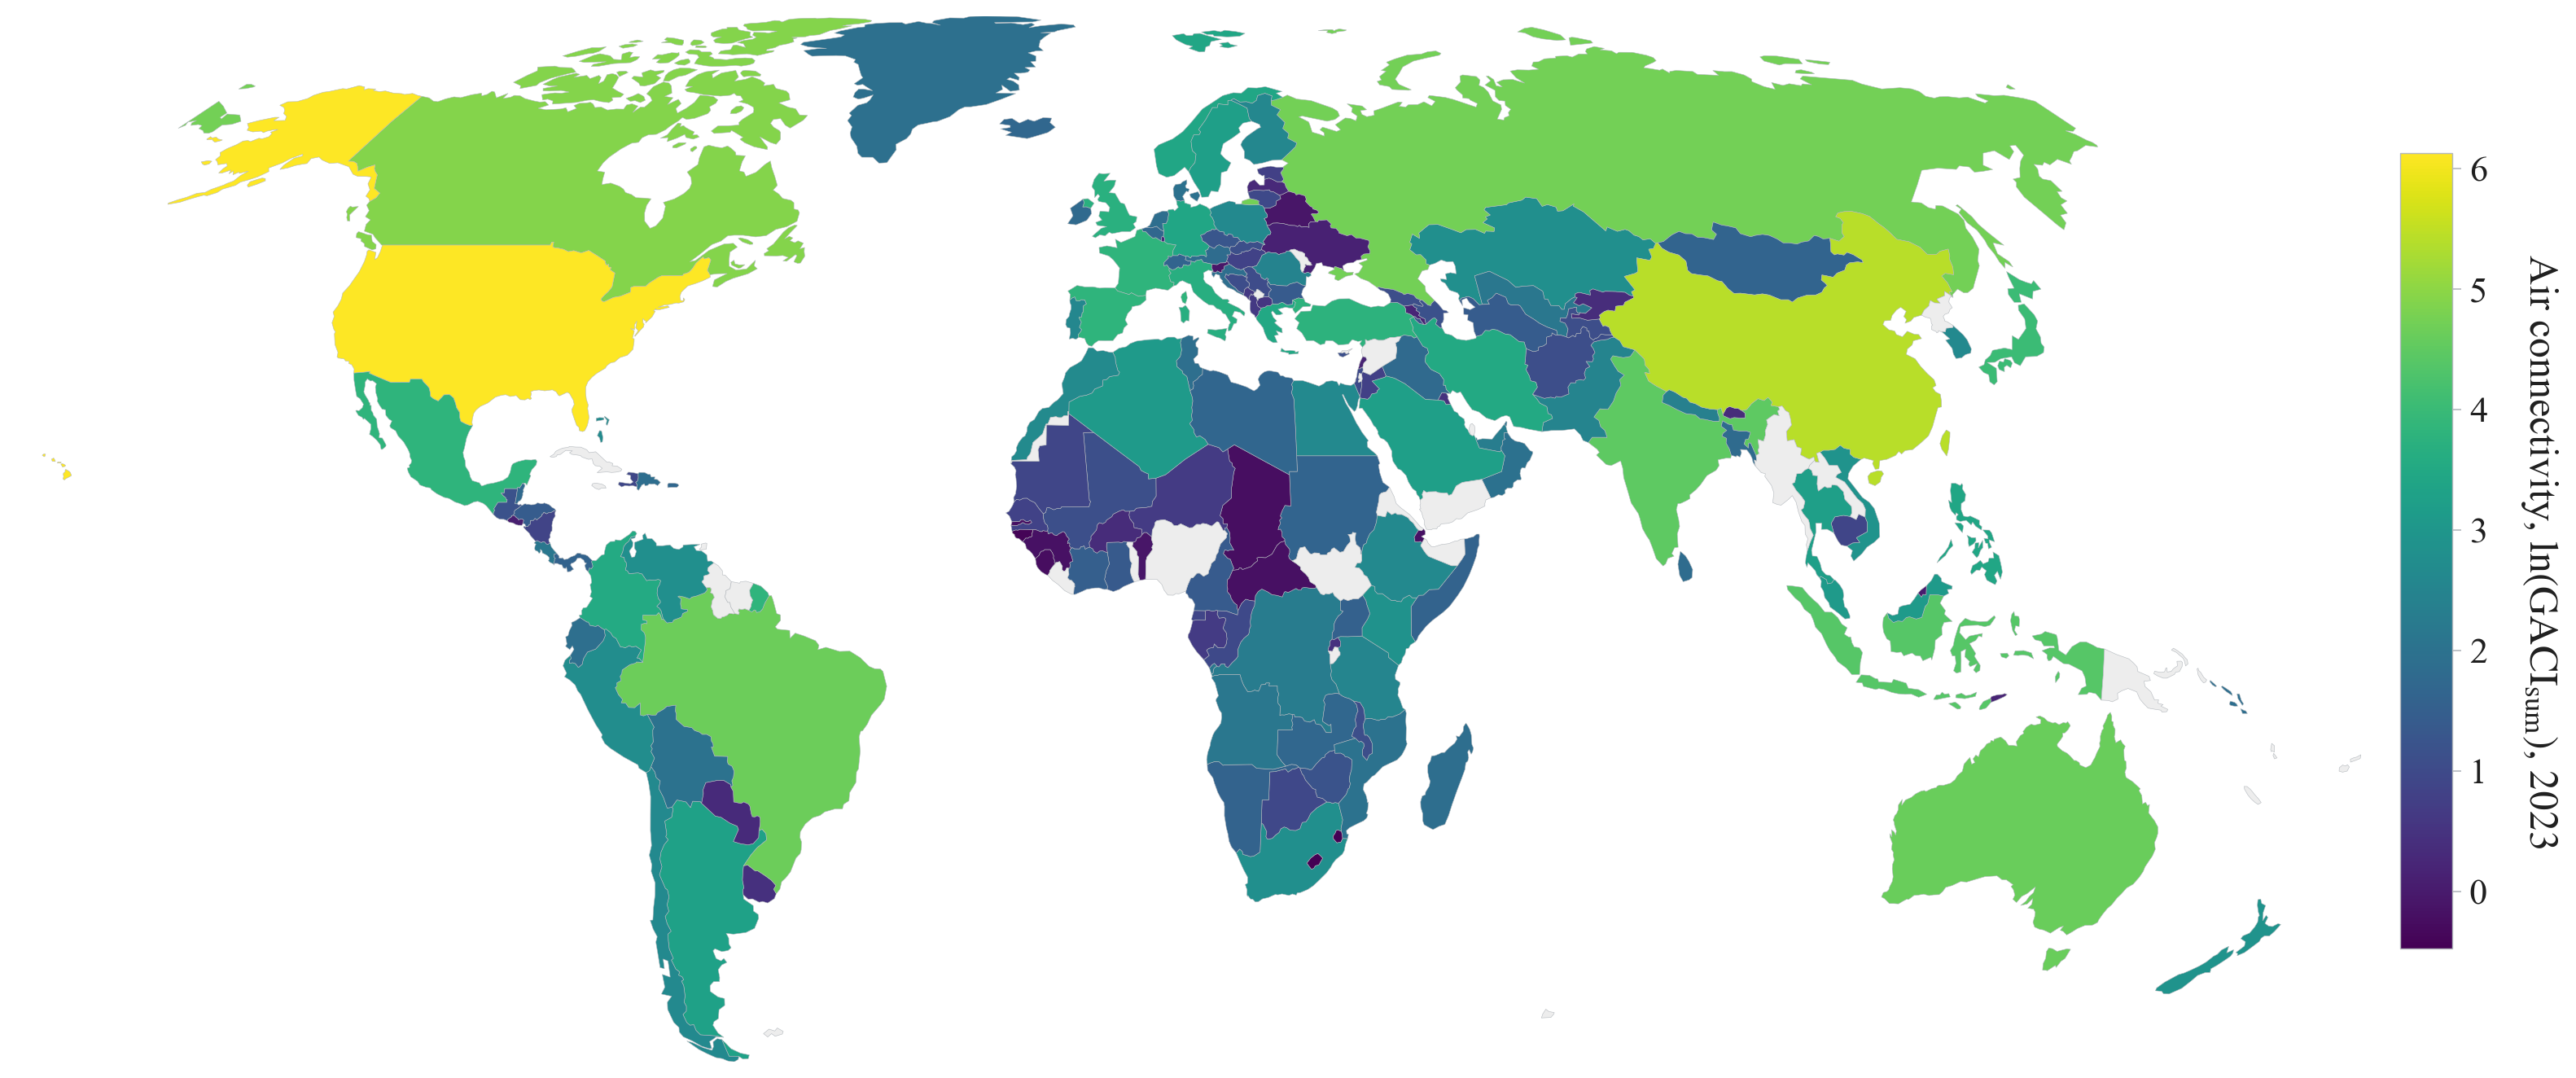
\includegraphics[width=0.9\linewidth]{GACI_base_map.png}
\caption{Air connectivity (GACI) levels, 2023. Yellow = highly connected
(United States, China, large European hubs).}
\label{fig:basemap}
\end{figure}
%=======================================================================
\section{Empirical strategy}
\label{sec:strategy}
% [Junya]
%=======================================================================
We estimate
\begin{equation}
y_{it} = \beta\,\ln\mathrm{GACI}_{it} + \gamma\,\ln\text{pop}_{it}
+ \alpha_i + \delta_t + \varepsilon_{it},
\label{eq:main}
\end{equation}
with country ($\alpha_i$) and year ($\delta_t$) fixed effects, instrumenting
$\ln\mathrm{GACI}_{it}$ by Eq.~\eqref{eq:instr}.

Identifying the causal effect of connectivity on trade is difficult for two
reasons. First, connectivity is poorly represented by a binary treatment. New
airports and major international routes open only rarely and lumpily, and a
country's effective network position evolves continuously---through
frequencies, partner growth, and re-routing---rather than through discrete,
datable openings; the discrete events that could anchor a staggered
difference-in-differences design are both scarce and a coarse proxy for the
connectivity that actually changes. Second, the variation that does exist is
endogenous: airlines add capacity where trade and income are already growing.
We address both with a continuous, network-based index that embeds second-order
(partner-of-partner) spillovers, instrumented by a shift-share interaction
\citep{GoldsmithPinkham_2020,Borusyak_2022} of a fixed heritage endowment with
the global tourism cycle. Heritage-driven leisure demand shifts an airport's
network position for reasons unrelated to goods-trade fundamentals, while the
outcome excludes services and tourism by construction. We report
heteroskedasticity-robust standard errors and probe the exclusion restriction
directly through over-identification (Section~\ref{sec:robust}).

Two extensions of Eq.~\eqref{eq:main} carry the rest of the paper. For the
mechanism analysis, we replace the outcome with composition measures built
from product-level trade and, in a second step, add those measures as controls
(Section~\ref{sec:mechanism}). For the aggregate accounting, we convert the
estimated openness elasticity into implied dollar magnitudes country by
country (Section~\ref{sec:aggregate}).

%=======================================================================
\section{Main results}
\label{sec:results}
%=======================================================================

WWe first ask whether global aviation connectivity raised trade openness, trade
volume, and GDP. Table~\ref{tab:main} reports, for each of our three measures of
global aviation connectivity, three lines side by side: the OLS association, the
first-stage relevance of the instrument, and the instrumented (2SLS) estimate.
Reading down each panel shows how isolating exogenous variation changes the
picture. The three measures agree closely in sign and significance, so we adopt
hub quality ($\ln\mathrm{GACI}_{cwm}$) as our main explanatory variable: unlike
the maximum, which discards every airport but the primary gateway, and the simple
sum, which weights a minor regional field the same as a major hub, the
capacity-weighted mean uses the entire airport system while still placing most
weight on the dominant hubs. We therefore report hub quality in Panel~A and treat
the maximum and the sum as robustness measures.

Panel A uses hub quality ($\ln\mathrm{GACI}_{cwm}$), our headline measure. The
instrument is a strong predictor of connectivity: it enters the first stage with
the expected positive sign ($0.032$, $p<0.01$), and the Kleibergen--Paap
statistic ($F=18.0$) sits comfortably above conventional weak-instrument
thresholds. In the second stage, a one-percent increase in hub quality raises
trade volume by about $2.3\%$ ($p<0.01$). This volume response decomposes into two
parts. Trade openness, the ratio of trade to GDP, rises by about $1.3\%$
($p<0.05$), and GDP rises by about $1.0\%$, although the GDP estimate is not
statistically significant. We treat trade openness as the headline result because
it isolates the pure trade effect net of economic scale: it measures whether
connectivity makes a country trade more relative to the size of its economy,
rather than simply enlarging the economy as a whole.

Panel B introduces the maximum hub measure ($\ln\mathrm{GACI}_{max}$), which keeps
only each country's single best-connected gateway. This is the strongest of the
three instruments: the tourism-heritage instrument enters the first stage at
$0.044$ ($p<0.01$) with a Kleibergen--Paap statistic of $27.4$, the highest in the
table. The second-stage estimates track Panel A in sign and significance, trade
volume rising by about $1.7\%$ ($p<0.01$) and openness by about $1.0\%$
($p<0.05$), while the GDP effect is again positive but not significant. That the
hub-only measure delivers the tightest first stage is consistent with the
hub-and-spoke logic that a country's primary gateway carries most of its
exogenous, tourism-driven connectivity.

Panel C repeats the exercise with total connectivity ($\ln\mathrm{GACI}_{sum}$),
which sums connectivity across all airports and so blends hub quality with sheer
airport count. The qualitative picture is unchanged: volume and openness are
positive and significant, while the GDP effect is positive but imprecise. Its
first stage is the weakest of the three ($F=9.7$), as expected once hub
concentration is diluted by peripheral airports. The three measures are on
different scales and cannot be compared coefficient for coefficient; what carries
over is the common pattern of signs and significance, together with the exact
decomposition that holds in every panel.

\begin{table}[ht!]
\centering
\caption{Main results: OLS, first stage, and 2SLS, by connectivity measure (robust SE).}
\label{tab:main}
\begin{threeparttable}
\small
\begin{tabular}{lccc}
\toprule
 & Trade openness & Trade volume & GDP \\
 & $\ln(g/Y)$ & $\ln g$ & $\ln Y$ \\
\midrule
\multicolumn{4}{l}{\emph{Panel A. Hub quality, $\ln\mathrm{GACI}_{cwm}$ (headline)}}\\
First stage: instrument coef. & \multicolumn{3}{l}{0.032\sym{***}\ \ (0.007),\ \ KP $F=18.0$} \\
OLS & 0.157\sym{***} & 1.144\sym{***} & 0.987\sym{***} \\
2SLS & 1.302\sym{**} & 2.303\sym{***} & 1.001 \\
 & (0.662) & (0.776) & (0.680) \\
\addlinespace
\multicolumn{4}{l}{\emph{Panel B. Maximum hub, $\ln\mathrm{GACI}_{max}$}}\\
First stage: instrument coef. & \multicolumn{3}{l}{0.044\sym{***}\ \ (0.008),\ \ KP $F=27.4$} \\
OLS & 0.103\sym{**} & 1.083\sym{***} & 0.980\sym{***} \\
2SLS & 0.966\sym{**} & 1.709\sym{***} & 0.743 \\
 & (0.469) & (0.548) & (0.507) \\
\addlinespace
\multicolumn{4}{l}{\emph{Panel C. Total connectivity, $\ln\mathrm{GACI}_{sum}$}}\\
First stage: instrument coef. & \multicolumn{3}{l}{0.064\sym{***}\ \ (0.020),\ \ KP $F=9.7$} \\
OLS & -0.027 & 0.237\sym{***} & 0.264\sym{***} \\
2SLS & 0.659\sym{*} & 1.166\sym{***} & 0.507 \\
 & (0.365) & (0.432) & (0.341) \\
\midrule
Country, Year FE & Yes & Yes & Yes \\
Observations & 4{,}642 & 4{,}642 & 4{,}642 \\
\bottomrule
\end{tabular}
\begin{tablenotes}\footnotesize
\item Robust (heteroskedasticity-consistent) SE in parentheses. Each panel
instruments its connectivity measure with the tourism-heritage instrument. The
first-stage row regresses the connectivity measure on the instrument (with
population and two-way FE); KP $F$ is the Kleibergen--Paap first-stage statistic.
Trade volume $=$ openness $+$ GDP by the identity $\ln g=\ln(g/Y)+\ln Y$.
\sym{*}~$p<0.10$, \sym{**}~$p<0.05$, \sym{***}~$p<0.01$.
\end{tablenotes}
\end{threeparttable}
\end{table}
%=======================================================================
\subsection{Heterogeneity: who gains most?}
%=======================================================================

We next ask whether the average effect masks variation in who benefits, letting
the connectivity elasticity vary with three mean-centred baseline moderators:
income (log GDP per capita), global aviation connectivity ($\ln\mathrm{GACI}_{cwm}$),
and remoteness. Remoteness is each country's unweighted mean sea distance to all
other sample countries, from the CERDI sea-distance database, in logs; it is a
time-invariant, purely geographic measure (we use the unweighted mean because
GDP-weighting collapses to market proximity and inverts the ranking).
Table~\ref{tab:het} reports interaction-IV estimates: for each moderator,
``$\ln\mathrm{GACI}_{cwm}$ (at mean)'' is the effect for the average country and
``$\times$ moderator'' is how that effect shifts as the moderator rises, with both
the connectivity term and its interaction instrumented.

The interactions with baseline income and baseline connectivity are negative and
significant across all three outcomes: the payoff to connectivity is larger in
poorer and less-connected economies. Remoteness works the same way for openness
(more remote economies gain more in trade intensity) but is imprecise for volume
and GDP. Evaluated at the mean the effect remains positive and sizeable. The
interacted first stages are weaker (KP $F\approx5$--$9$), so we read the gradient
as a qualitative pattern and report every cell.

\begin{table}[ht!]
\centering
\caption{Heterogeneity: interaction IV (robust SE).}
\label{tab:het}
\begin{threeparttable}
\small
\begin{tabular}{lccc}
\toprule
Moderator (mean-centred): & Baseline income & Baseline conn. & Remoteness \\
\midrule
\multicolumn{4}{l}{\emph{Panel A. Trade openness $\ln(g/Y)$}}\\
$\ln\mathrm{GACI}_{cwm}$ (at mean)   & 1.254\sym{*}  & 2.260\sym{*}  & 1.391\sym{**} \\
                         & (0.717)       & (1.161)       & (0.693) \\
$\times$ moderator       & $-0.243$\sym{**} & $-1.482$\sym{**} & $-1.241$\sym{*} \\
                         & (0.122)       & (0.622)       & (0.673) \\
\addlinespace
\multicolumn{4}{l}{\emph{Panel B. Trade volume $\ln g$}}\\
$\ln\mathrm{GACI}_{cwm}$ (at mean)   & 1.959\sym{***} & 6.093\sym{***} & 2.394\sym{***} \\
                         & (0.732)       & (1.742)       & (0.825) \\
$\times$ moderator       & $-1.108$\sym{***} & $-6.060$\sym{***} & $-1.234$ \\
                         & (0.131)       & (1.046)       & (0.815) \\
\addlinespace
\multicolumn{4}{l}{\emph{Panel C. GDP $\ln Y$}}\\
$\ln\mathrm{GACI}_{cwm}$ (at mean)   & 0.705         & 3.834\sym{***} & 1.003 \\
                         & (0.759)       & (1.133)       & (0.708) \\
$\times$ moderator       & $-0.865$\sym{***} & $-4.579$\sym{***} & 0.007 \\
                         & (0.119)       & (0.677)       & (0.755) \\
\midrule
First-stage KP $F$       & 8.07          & 4.96          & 9.21 \\
Country, Year FE         & Yes           & Yes           & Yes \\
Observations             & 4{,}121       & 4{,}121       & 4{,}635 \\
\bottomrule
\end{tabular}
\begin{tablenotes}\footnotesize
\item Each column is one moderator. Both $\ln\mathrm{GACI}_{cwm}$ and its
interaction with the (mean-centred) moderator are instrumented; country and year
FE; robust SE. Negative interactions on income and baseline connectivity
(significant across all three outcomes) mean the payoff is larger for poorer and
less-connected economies. KP $F$ is modest ($\approx5$--$9$), so the gradient is
qualitative. All cells reported, including the insignificant ones.
\sym{*}~$p<0.10$, \sym{**}~$p<0.05$, \sym{***}~$p<0.01$.
\end{tablenotes}
\end{threeparttable}
\end{table}

Figure~\ref{fig:hetquartile} makes this gradient concrete by plotting the implied
openness elasticity for each quartile of baseline income and baseline
connectivity. In both dimensions the elasticity falls monotonically from the
lowest to the highest quartile, from about $1.7$ to $0.8$ across income quartiles
and from about $2.7$ to $1.7$ across connectivity quartiles, though the confidence
intervals are wide, consistent with reading the pattern as qualitative.

\begin{figure}[ht!]
\centering
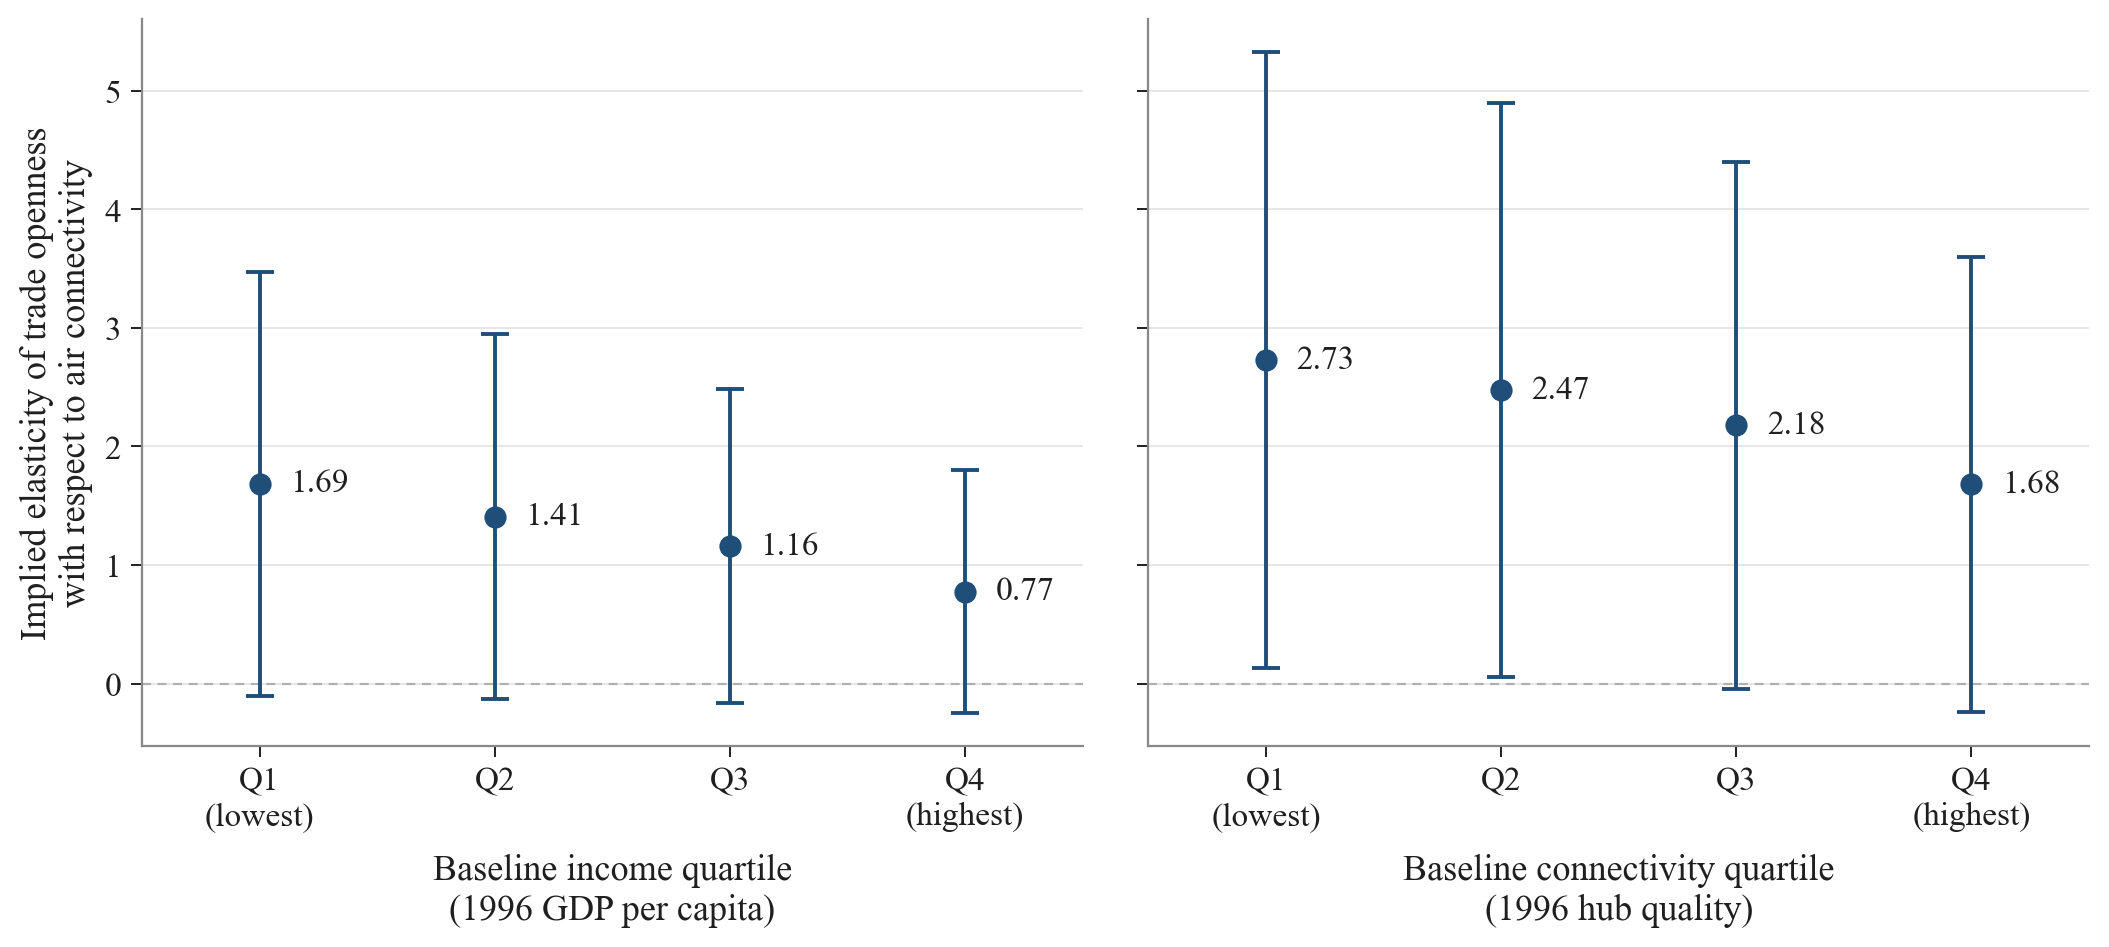
\includegraphics[width=0.95\linewidth]{GACI_hetero_quartile.png}
\caption{Implied elasticity of trade openness with respect to global aviation
connectivity, by baseline-income and baseline-connectivity quartile (Q1 = lowest;
95\% CIs).}
\label{fig:hetquartile}
\end{figure}

%=======================================================================
\subsection{Temporal heterogeneity}
\label{sec:temporal}
%=======================================================================
We also examine whether the effect has shifted over time by interacting
$\ln\mathrm{GACI}_{cwm}$ with a post-2010 indicator (Table~\ref{tab:temporal}).
The table reports the pre-2010 effect and how it changes after 2010 for each
outcome. The instrument is essentially irrelevant before 2010 (first-stage KP
$F=0.29$) and strong afterwards ($F=27.7$), so identification comes almost
entirely from the recent period. Consistent with this, the post-2010 shift is
positive and significant for volume and GDP: the impact is concentrated in the
post-2010 era of low-cost long-haul and Gulf and Asian hub expansion.

\begin{table}[ht!]
\centering
\caption{Temporal heterogeneity: interaction with post-2010 (robust SE).}
\label{tab:temporal}
\begin{threeparttable}
\small
\begin{tabular}{lccc}
\toprule
 & Trade openness & Trade volume & GDP \\
\midrule
$\ln\mathrm{GACI}_{cwm}$ (pre-2010) & 1.247   & 0.496   & $-0.751$ \\
                        & (0.771) & (0.877) & (0.983) \\
$\times$ post-2010      & 0.012   & 0.377\sym{***} & 0.366\sym{***} \\
                        & (0.076) & (0.088) & (0.091) \\
\midrule
Country, Year FE        & Yes & Yes & Yes \\
\bottomrule
\end{tabular}
\begin{tablenotes}\footnotesize
\item Country and year FE; robust SE. The instrument is essentially irrelevant
before 2010 (first-stage KP $F=0.29$) and strong afterwards ($F=27.7$), so
identification is concentrated in the post-2010 period; the effect on volume
and GDP is significantly larger after 2010.
\sym{*}~$p<0.10$, \sym{**}~$p<0.05$, \sym{***}~$p<0.01$.
\end{tablenotes}
\end{threeparttable}
\end{table}

%=======================================================================
\subsection{Mechanism: composition carries the openness effect}
\label{sec:mechanism}
\label{sec:mediation}
%=======================================================================
The conceptual framework in Section~\ref{sec:framework} predicts that if
connectivity works through high-value air cargo and value-chain
participation, it should change the \emph{mix} of trade, and that this
compositional change should carry the openness effect.
Table~\ref{tab:mechanism} tests both steps with two composition measures
built from BACI product-level data (Section~\ref{sec:data}): the log
ratio of intermediate to consumption goods, the value-chain margin, and
the log ratio of high to low unit-value trade, the air-freight margin.
Ratios net out shocks common to all of a country's trade, so they move
only when the trade mix moves.

The first step asks whether connectivity changes the trade mix, taking
each composition ratio as the outcome. It does: a rise in hub quality
shifts trade toward high value-to-weight goods (column (4): $1.71$,
$p<0.05$), and the shift toward intermediate goods points the same way
(column (2): $1.12$, s.e.\ $0.69$). Connectivity does not raise all
trade proportionally; it tilts the basket toward the goods that air
transport serves.

The second step asks whether this compositional change carries the
openness effect. The logic is a comparison across columns: if
connectivity raised openness through some channel unrelated to
composition, its coefficient should be unchanged when the composition
ratios enter the openness regression as controls; if the effect operates
through composition, the coefficient should fall toward zero while the
ratios absorb it. The data choose the second reading. The connectivity
coefficient falls from $1.27$ in column (1) to $1.09$ when the
intermediates ratio enters (column (3)) and to $1.00$---no longer
statistically distinguishable from zero---when both ratios enter (column
(6)). The composition ratios themselves are strong predictors of
openness throughout: a trade basket tilted toward intermediates and
high-value goods is a more open one (column (6): $0.173$, $p<0.01$ and
$0.047$, $p<0.05$). The sample is identical in every column, so the
decline of the connectivity coefficient reflects the controls, not the
data. Taken together, the two steps close the loop: connectivity
re-composes trade toward air-served goods, and that re-composition
accounts for the openness effect.

\begin{table}[t]
\centering
\caption{Mechanism: connectivity, trade composition, and openness, 2SLS,
1996--2023.}
\label{tab:mechanism}
\begin{threeparttable}
\small
\begin{tabular}{lcccccc}
\toprule
 & (1) & (2) & (3) & (4) & (5) & (6) \\
Dependent variable: & Openness & $\ln\frac{\text{Interm.}}{\text{Consum.}}$ & Openness & $\ln\frac{\text{High VW}}{\text{Low VW}}$ & Openness & Openness \\
\midrule
$\ln\mathrm{GACI}_{cwm}$ & 1.268\sym{*} & 1.116 & 1.086\sym{*} & 1.714\sym{**} & 1.247\sym{*} & 0.996 \\
 & (0.656) & (0.693) & (0.638) & (0.753) & (0.668) & (0.649) \\
ln(Interm./Consum.) &  &  & 0.163\sym{***} &  &  & 0.173\sym{***} \\
 &  &  & (0.019) &  &  & (0.019) \\
ln(High/Low VW) &  &  &  &  & 0.012 & 0.047\sym{**} \\
 &  &  &  &  & (0.021) & (0.020) \\
\midrule
First-stage KP $F$ & 18.1 & 18.1 & 17.7 & 18.1 & 17.5 & 16.9 \\
Observations & 4614 & 4614 & 4614 & 4614 & 4614 & 4614 \\
\bottomrule
\end{tabular}
\begin{tablenotes}\footnotesize
\item Notes: Robust standard errors in parentheses. *, **, *** denote
significance at the 10\%, 5\%, and 1\% levels, respectively.
\item Openness is $\ln(\text{trade}/\text{GDP})$. The composition ratios
are built from BACI HS92 bilateral product-level data aggregated to
country-year values (exports plus imports): intermediate versus
consumption goods by BEC end-use, and high versus low unit-value trade
split at the pooled product median (USD/kg). All columns instrument
$\ln\mathrm{GACI}_{cwm}$ with the tourism-heritage instrument and include
country and year fixed effects and $\ln$ population, as in
Table~\ref{tab:main}. Columns (2) and (4) take the composition ratios as
outcomes (does connectivity change the trade mix?); columns (3), (5),
and (6) add them as controls (does the change in mix carry the openness
effect?). Column (1) differs marginally from Table~\ref{tab:main}
because the sample requires nonmissing composition ratios.
\end{tablenotes}
\end{threeparttable}
\end{table}

%=======================================================================
\subsection{Aggregate contribution of connectivity growth, 1996--2023}
\label{sec:aggregate}
%=======================================================================
The elasticity in Table~\ref{tab:main} on its own says little about how much trade
is at stake. We therefore translate it into an aggregate magnitude. This serves
two purposes: it expresses the estimate in units that matter for policy (dollars
of trade and points of GDP), and it lets the contribution of two decades of global
aviation connectivity growth be compared against the size of the world economy.

The calculation is a partial-equilibrium counterfactual. For each country we ask
how much of its 2023 trade is attributable to that country's own 1996--2023 rise
in hub quality, holding everything else fixed. Applying the intensity (openness)
elasticity, the attributable share is
$1-\exp(-\beta\,\Delta\ln\mathrm{GACI}_{cwm,i})$ with $\beta=1.302$, so the
implied gain is
$\text{trade}_i\times\bigl(1-\exp(-\beta\,\Delta\ln\mathrm{GACI}_{cwm,i})\bigr)$;
summing across countries gives the world total.

On this basis, global aviation connectivity growth since 1996 is associated with
about \textbf{\$7.8 trillion} of 2023 trade, roughly \textbf{17\%} of 2023 world
trade (\$47 trillion) and \textbf{7.4\%} of 2023 world GDP, equivalently raising
world trade openness by about 7.4 percentage points of GDP. Figure~\ref{fig:continent}
traces the implied openness gain by continent over time and shows these gains
accrue most to the Middle East (Gulf hubs) and Asia (China), which pull away from
the rest after 2005.

\begin{figure}[ht!]
\centering
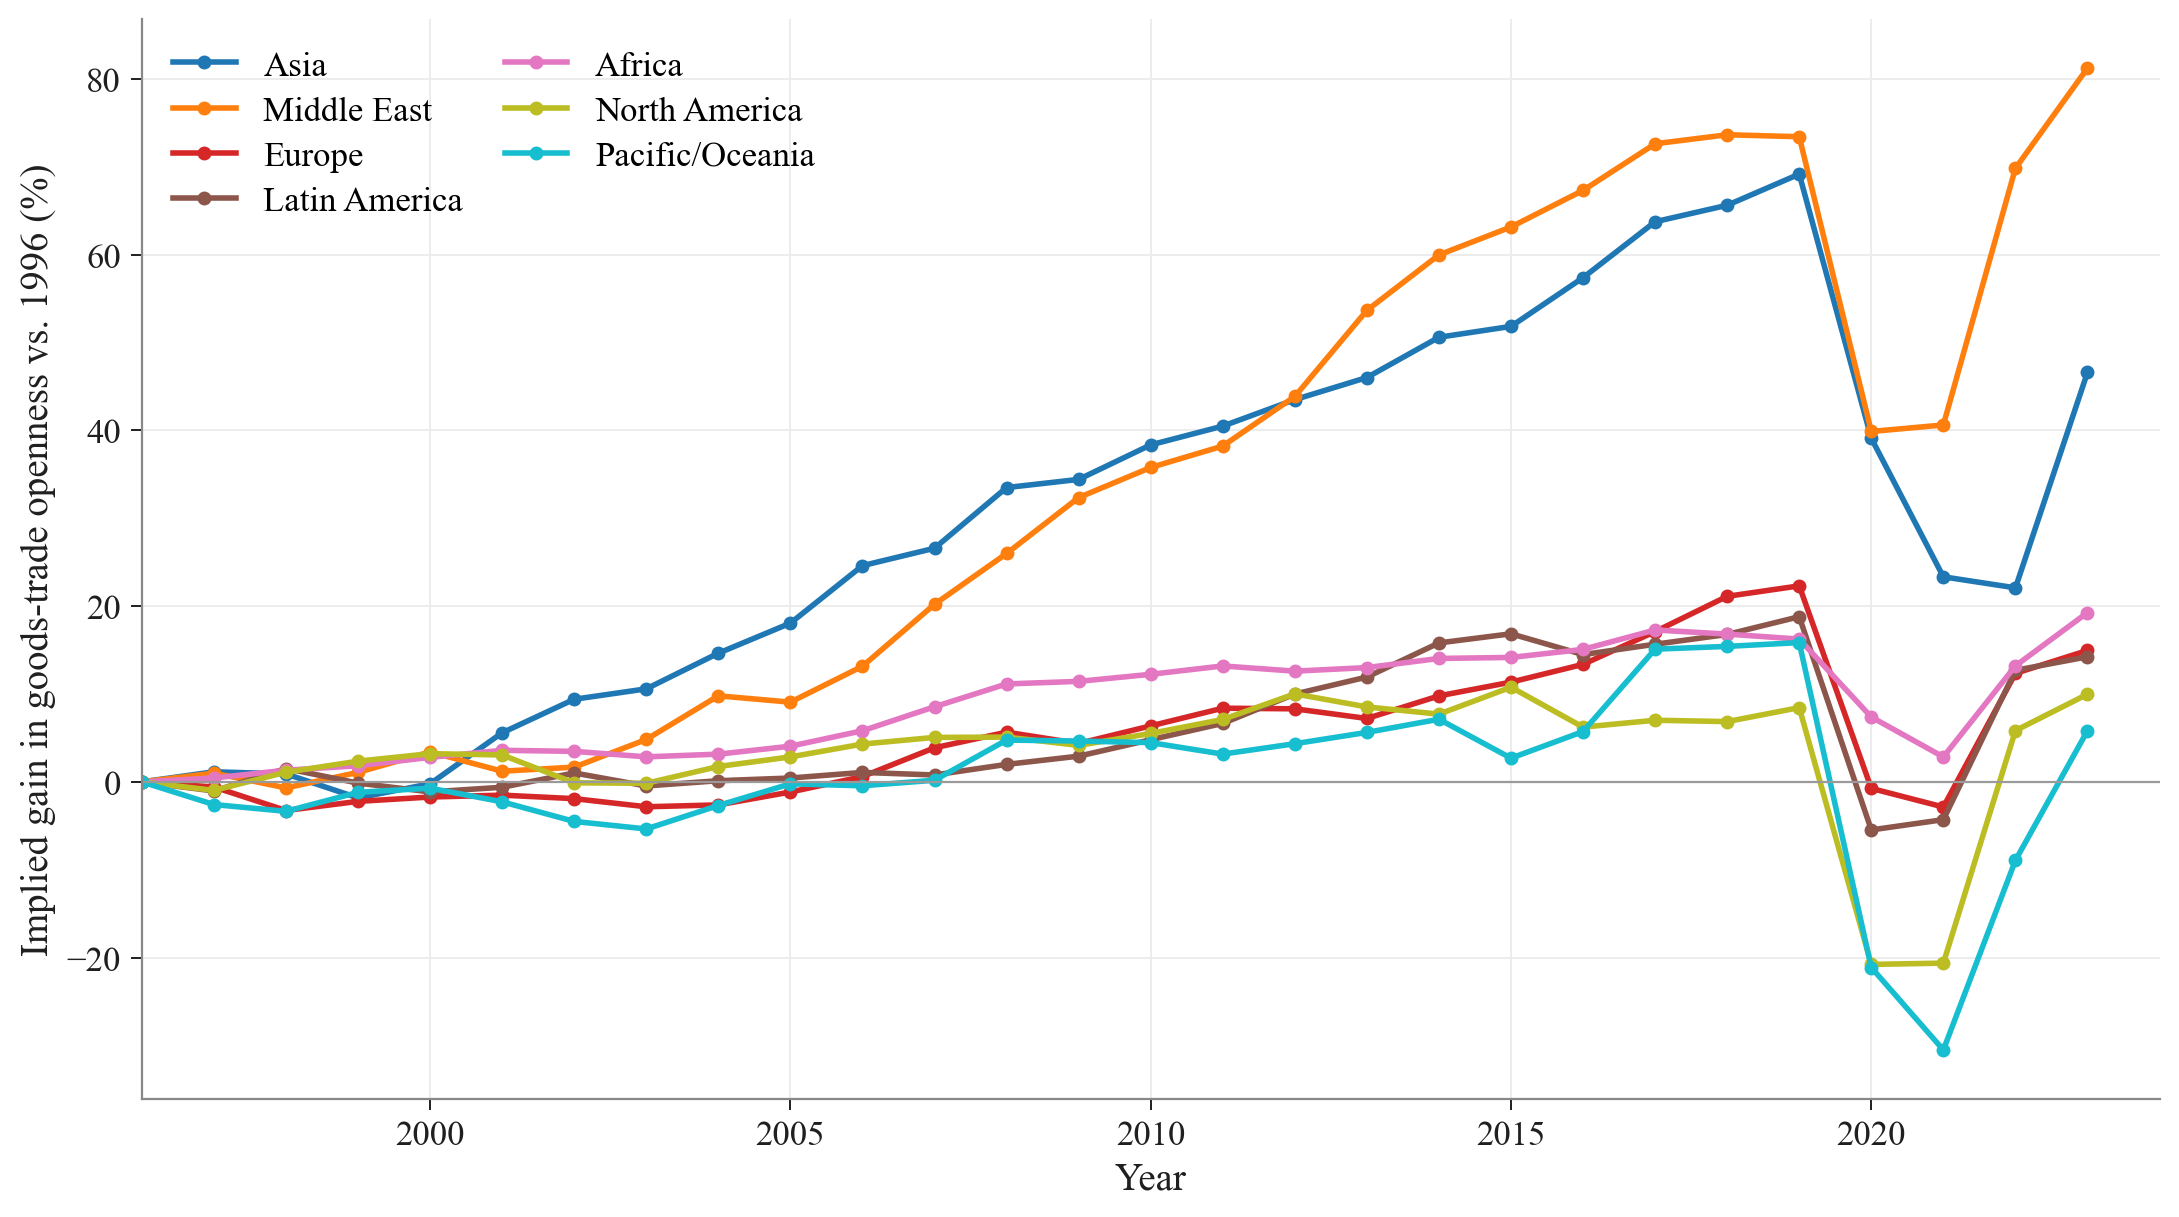
\includegraphics[width=0.9\linewidth]{GACI_continent_trend.png}
\caption{Implied gain in trade openness relative to 1996, by continent (intensity
channel, $\beta=1.302$).}
\label{fig:continent}
\end{figure}

The headline figure uses hub quality ($\mathrm{GACI}_{cwm}$), but the magnitude is
not an artefact of that choice. Table~\ref{tab:contribution} repeats the
counterfactual for all three national connectivity aggregations (the
seat-capacity-weighted mean used in the headline, the single largest hub, and the sum
of airport indices), each with its own estimated elasticity. The implied trade contribution is strikingly stable: the
intensity channel attributes \$6.8--7.8 trillion of 2023 goods trade (14.5--16.5\% of
the world total), and the volume channel \$10.2--11.5 trillion (21.6--24.6\%),
regardless of measure. This stability is not mechanical, because the measures with
larger elasticities (hub quality) also display smaller log-changes over the period,
so the two offset. Applying the GDP-scale elasticity to GDP levels implies a further
\$9.8--13.2 trillion; we treat this as indicative only, since that elasticity is not
statistically distinguishable from zero.

\begin{table}[t]
\centering
\caption{Aggregate contribution of aviation-connectivity growth, 1996--2023, under
three connectivity measures.}
\label{tab:contribution}
\begin{threeparttable}
\small
\begin{tabular}{lcccccc}
\toprule
 & \multicolumn{2}{c}{Trade, intensity} & \multicolumn{2}{c}{Trade, volume}
 & \multicolumn{2}{c}{GDP, scale} \\
\cmidrule(lr){2-3}\cmidrule(lr){4-5}\cmidrule(lr){6-7}
Measure & $\beta_{\text{int}}$ & \$tn\,(\%\,wT) & $\beta_{\text{vol}}$ & \$tn\,(\%\,wT)
 & $\beta_{\text{GDP}}$ & \$tn\,(\%\,Y) \\
\midrule
$\mathrm{GACI}_{cwm}$ (headline) & 1.302 & 7.8\ (16.5) & 2.303 & 11.5\ (24.6) & 1.001 & 13.2\ (12.6) \\
$\mathrm{GACI}_{max}$ & 0.966 & 6.8\ (14.5) & 1.709 & 10.2\ (21.6) & 0.743 & \phantom{0}9.8\ (\phantom{0}9.4) \\
$\mathrm{GACI}_{sum}$ & 0.659 & 7.5\ (16.0) & 1.166 & 10.5\ (22.4) & 0.507 & 13.0\ (12.5) \\
\bottomrule
\end{tabular}
\begin{tablenotes}\footnotesize
\item Notes: Each dollar cell is the world sum of country-level attributable gains,
$\sum_i \text{level}_i(2023)\times[1-\exp(-\beta\,\Delta\ln\mathrm{GACI}_i)]$, where
$\beta$ is the corresponding 2SLS elasticity and $\Delta\ln\mathrm{GACI}_i$ is the
country's 1996--2023 change in that measure. ``Intensity'' applies the openness
elasticity to goods-trade levels (headline); ``volume'' applies the trade-volume
elasticity (an upper bound that folds in the GDP-scale channel); ``GDP, scale''
applies the GDP elasticity to GDP levels. World bases are 2023 goods trade
(\$46.9~trillion) and GDP (\$104.6~trillion); \%\,wT is the share of world goods
trade and \%\,Y the share of world GDP. The trade-volume elasticities are significant
at 1\% for all three measures; the openness elasticities at 5\% (max, cwm) and 10\%
(sum); the GDP elasticities are not statistically significant, so the GDP columns are
indicative only.
\end{tablenotes}
\end{threeparttable}
\end{table}

\begin{figure}[ht!]
\centering
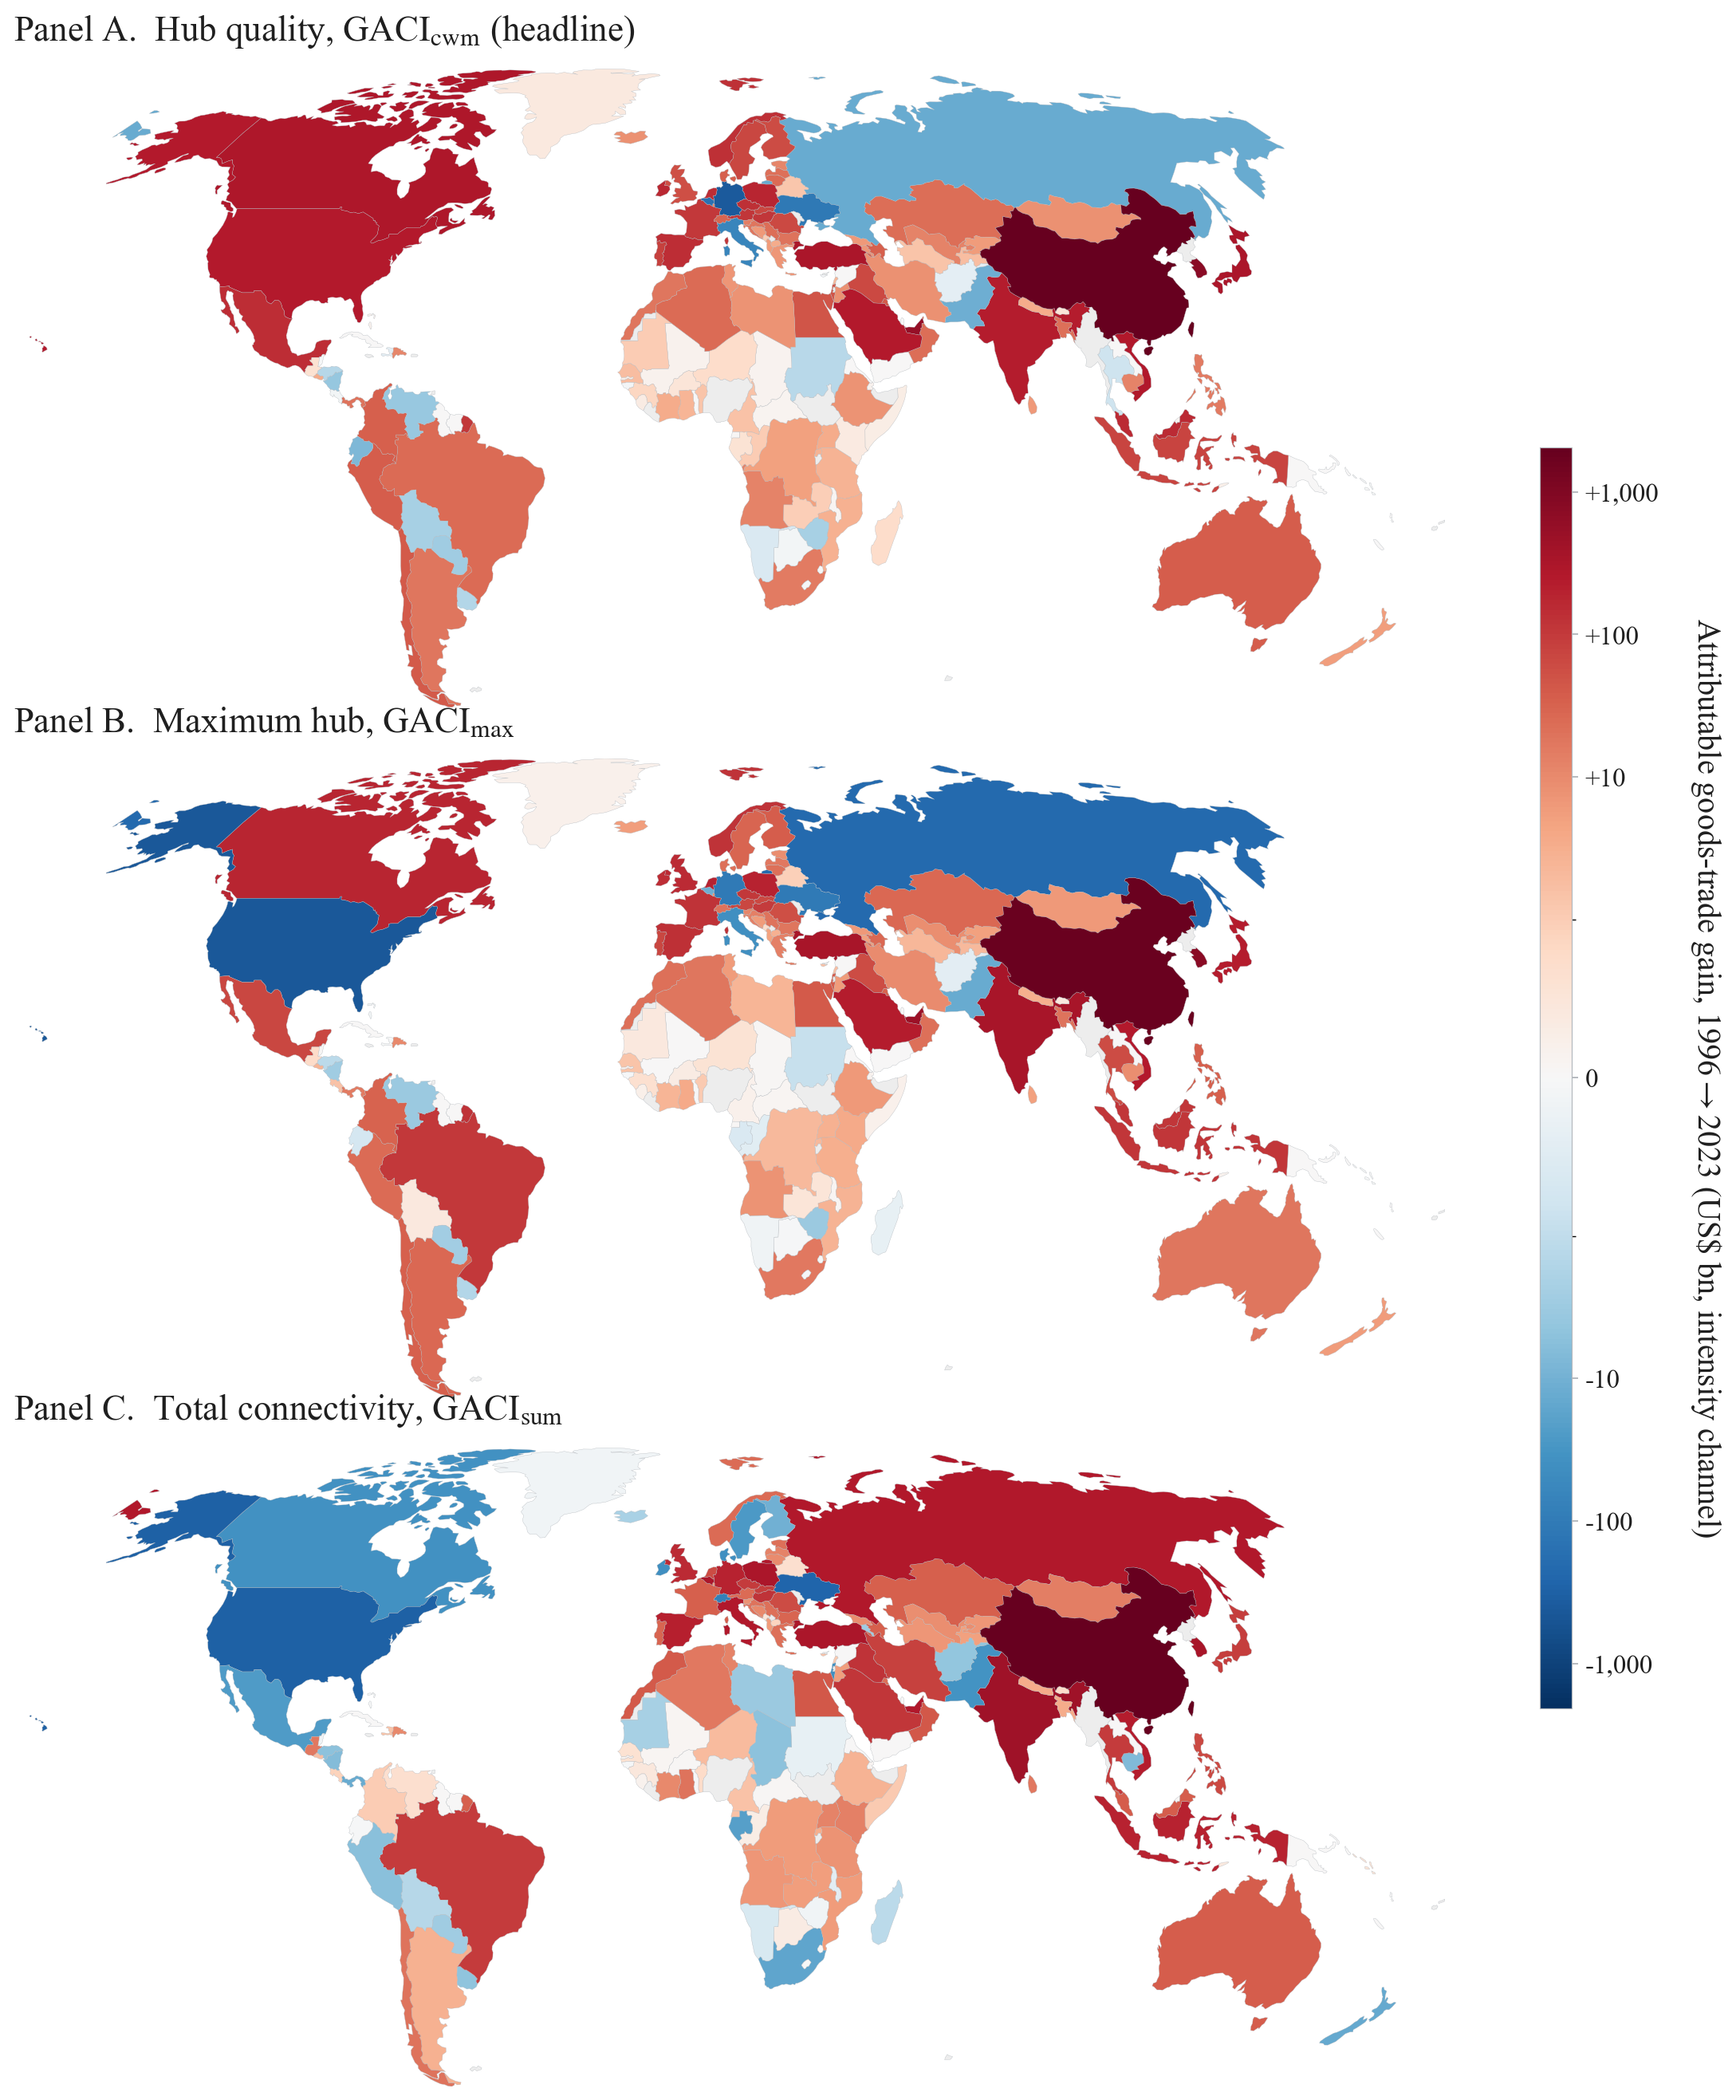
\includegraphics[width=\linewidth]{GACI_contrib_trade_3panel.png}
\caption{Country-level contribution of aviation-connectivity growth to goods trade,
1996--2023 (intensity channel), under the three connectivity measures. Red denotes
positive attributable trade (connectivity rose), blue negative (connectivity fell on
that measure), and grey is outside the sample. Gains are dominated by China, India,
and emerging Asia; a sizeable minority of countries (42--60 of 184, depending on the
measure) saw connectivity fall over the period, so the world totals in
Table~\ref{tab:contribution} are net of these losses.}
\label{fig:contribmap}
\end{figure}

%=======================================================================
\subsection{Connectivity-collapse shocks}
%=======================================================================
The same logic applies in reverse: if global aviation connectivity raises trade on
the way up, an abrupt collapse should subtract it on the way down. We apply the
counterfactual to the COVID-19 collapse (2019 to 2020) for all three measures,
keeping hub quality ($\mathrm{GACI}_{cwm}$) as the headline for consistency with the
rest of the paper. Connectivity fell in 154 of 175 countries on the hub-quality
measure (median $\Delta\ln\mathrm{GACI}_{cwm}=-0.073$), implying a one-year
goods-trade disruption of about \$7.5 trillion, roughly 20\% of 2019 world trade; the
maximum-hub measure implies \$6.7 trillion (18\%), and total connectivity
\$1.8 trillion (4.8\%). The corresponding GDP contraction ranges from \$2.5 trillion
(total connectivity) to \$13.2 trillion (hub quality), about 3 to 15\% of 2019 world
GDP, though it rests on the imprecise GDP elasticities and is only indicative. Two
cautions attach to these magnitudes. First, the
elasticities are long-run cross-country estimates, so applying them to a single year
overstates the short-run response: the hub-quality figure is best read as an
illustrative upper bound and the sum-based figure as a conservative lower bound.
Second, in 2020 connectivity and trade fell together under a common shock (pandemic
demand and lockdowns), so the exercise attributes to connectivity a contraction that
has other causes as well. With those caveats the direction is unambiguous: an abrupt
connectivity collapse subtracts trade, concentrated in the major gateway hubs that
had gained the most on the way up. Figure~\ref{fig:shock} maps the effect country by
country for each measure.

\begin{figure}[ht!]
\centering
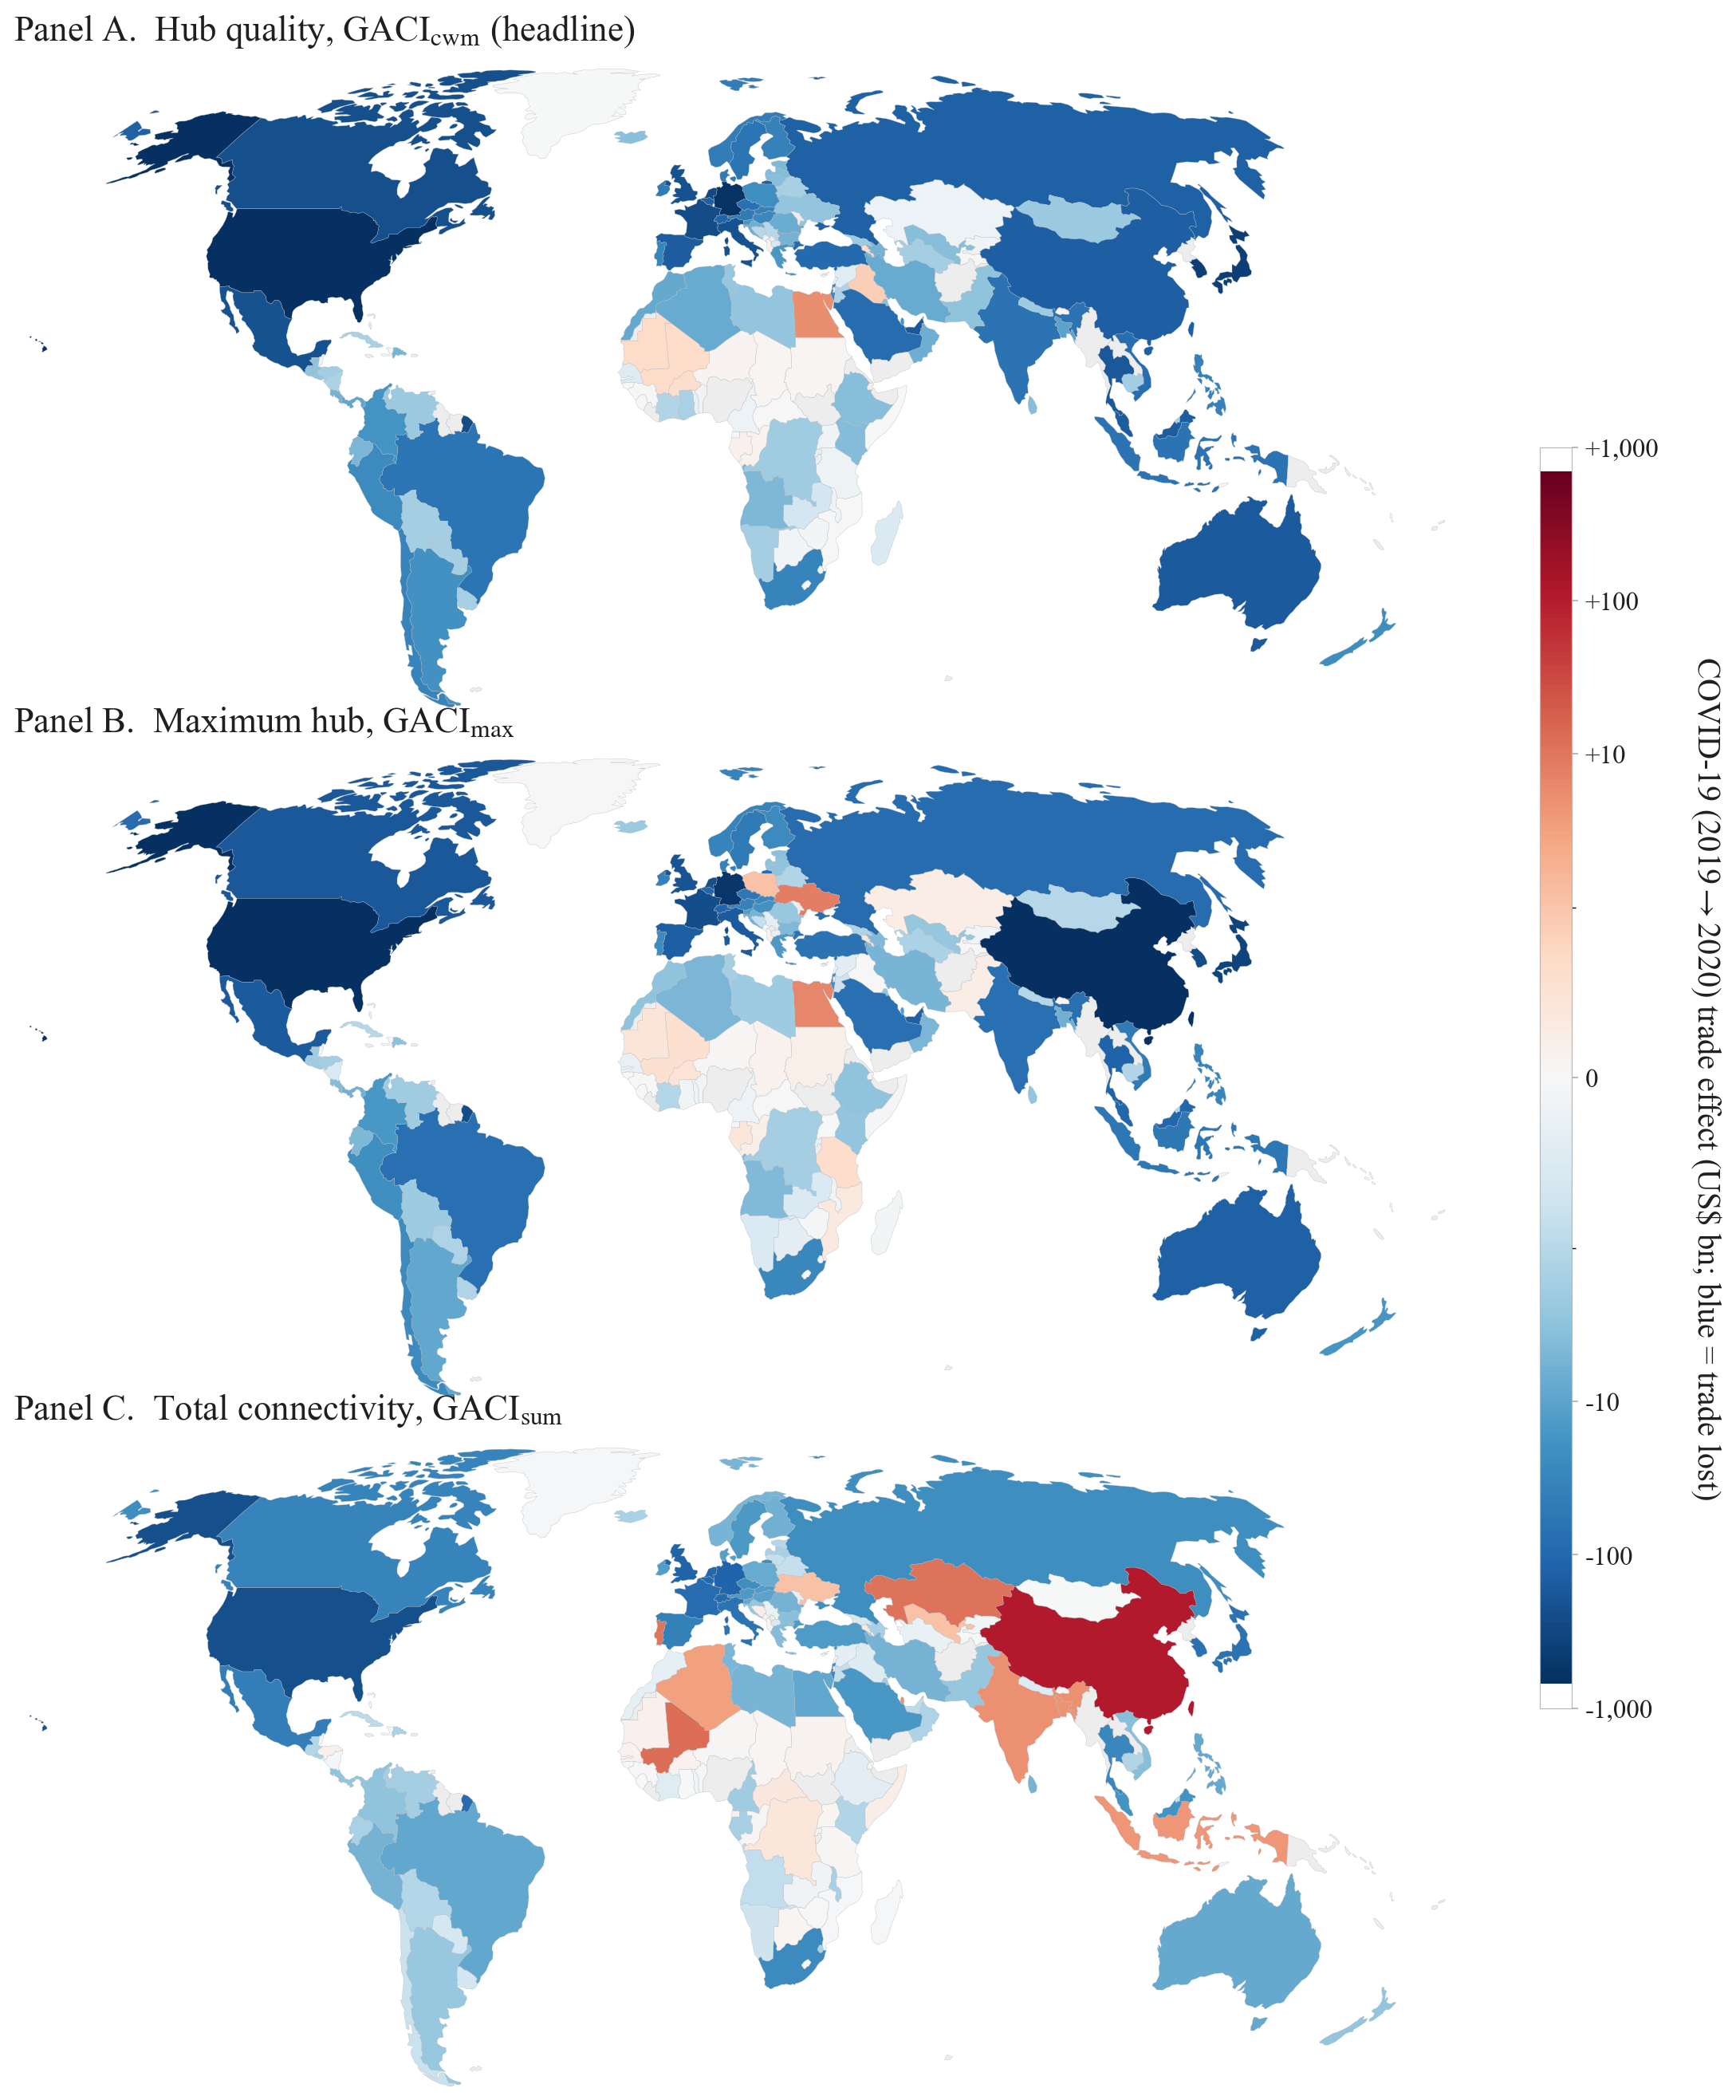
\includegraphics[width=\linewidth]{GACI_covid_shock_3panel.png}
\caption{COVID-19 (2019 to 2020): implied country-level goods-trade effect of the
aviation-connectivity collapse, under the three connectivity measures. Blue denotes
trade lost, red trade gained, and grey is outside the sample. The loss is broad and
concentrated in major gateway hubs; under total connectivity (Panel C) a few
countries register mechanical gains because their summed index rose over the year.}
\label{fig:shock}
\end{figure}

Taken together, these results carry four messages. First, global aviation
connectivity is a causal driver of trade integration, and it operates primarily on
the intensity margin: better-connected countries trade more relative to the size
of their economies, not merely because they are larger. Second, the effect works
through composition: connectivity tilts the trade mix toward high value-to-weight
and intermediate goods, and this shift carries the openness effect. Third, the
returns are unevenly shared and are largest for poorer, less-connected, and more
remote economies, so aviation acts as a convergence lever that substitutes for
weak surface and maritime access. Fourth, because connectivity builds trade on
the way up, abrupt collapses subtract it on the way down, as the COVID-19 episode
shows. The policy implication is direct: airport and route investment and
air-service liberalisation are concrete levers for trade integration, with the
highest marginal returns in peripheral economies.

%=======================================================================
\section{Instrument validity and robustness}
\label{sec:robust}
%=======================================================================
The exclusion restriction requires that heritage-driven tourism demand affects
goods trade only through air connectivity. Our design narrows the space of
violations from the outset: the outcome is merchandise trade, so the mechanical
channel from tourism to services exports is excluded by construction, and
country fixed effects absorb every time-invariant characteristic---geography,
coastline, colonial history---through which heritage endowments could otherwise
matter. This section probes what remains, in three steps: sensitivity to
controls, formal over-identification and falsification tests, and an
independent instrument.

\paragraph{Sensitivity to controls.} A first, simple check is whether the
estimate depends on what else is in the regression \citep[cf.][]{Frankel_1999}.
Because country fixed effects absorb all time-invariant controls, the feasible
time-varying candidates are population and income. Table~\ref{tab:controls}
re-estimates the headline openness regression under five control sets. The
estimate barely moves: $1.66$ with no controls, $1.30$ with population (the
baseline), $1.71$ with GDP, $1.64$ with both, and $1.43$ with population and
GDP per capita, always significant at the 5 per cent level, with the first
stage strong throughout (KP $F=15.1$--$20.9$). Note that GDP is itself an
outcome of connectivity (Table~\ref{tab:main}), so conditioning on it
over-controls; that the openness effect survives even this conservative check
is reassuring.

\begin{table}[t]
\centering
\caption{Sensitivity to controls: 2SLS effect of connectivity on trade
openness under alternative control sets.}
\label{tab:controls}
\begin{threeparttable}
\small
\begin{tabular}{lccccc}
\toprule
 & (1) & (2) & (3) & (4) & (5) \\
Controls: & None & $\ln$ pop.\ & $\ln$ GDP & $\ln$ pop.\ $+$ & $\ln$ pop.\ $+$ \\
 & & (baseline) & & $\ln$ GDP & $\ln$ GDP p.c.\ \\
\midrule
$\ln\mathrm{GACI}_{cwm}$ & 1.663\sym{**} & 1.302\sym{**} & 1.706\sym{**} & 1.642\sym{**} & 1.430\sym{**} \\
 & (0.775) & (0.662) & (0.688) & (0.686) & (0.704) \\
\midrule
First-stage KP $F$ & 15.1 & 18.0 & 19.1 & 18.9 & 20.9 \\
Observations & 4642 & 4642 & 4642 & 4642 & 4642 \\
\bottomrule
\end{tabular}
\begin{tablenotes}\footnotesize
\item Notes: Robust standard errors in parentheses. *, **, *** denote
significance at the 10\%, 5\%, and 1\% levels, respectively.
\item Dependent variable: trade openness, $\ln(\text{trade}/\text{GDP})$. All
columns instrument $\ln\mathrm{GACI}_{cwm}$ with the tourism-heritage
instrument and include country and year fixed effects; only the time-varying
controls differ. Column (2) is the baseline specification of
Table~\ref{tab:main}. GDP is itself an outcome of connectivity, so columns
(3)--(5) over-control; the stability of the estimate is a conservative check.
\end{tablenotes}
\end{threeparttable}
\end{table}

Table~\ref{tab:robust} collects the formal tests of the identifying assumption.

\paragraph{(A) Over-identification with natural and mixed heritage.} Entering
natural and mixed heritage as two \emph{separate} instruments over-identifies
the single endogenous regressor and licenses a Hansen $J$ test. The two
instruments agree: $J$ is far from rejection for every outcome, and the volume
elasticity is essentially unchanged ($2.18$, $p<0.01$). The first stage remains
adequate (KP $F=8.5$).

\paragraph{(B) Falsification: adding cultural heritage.} Cultural heritage
co-moves with development and historic urban and manufacturing centres, so it
is a plausible exclusion-violator. Adding it as a third instrument moves the
Hansen $J$ to rejection for the volume outcome ($p=0.004$) and collapses the
point estimate. The data thus \emph{reject} cultural heritage as a valid
instrument---exactly the discriminating result that supports restricting the
instrument to natural and mixed endowments.

\paragraph{(C) Independent air/sea-distance instrument.} As a fully independent
identification path we construct a Frankel--Romer/Feyrer-type predicted
air-linkage instrument from geography and the CERDI sea-distance database
\citep{Frankel_1999,Feyrer_2019,Bertoli_2016}. Used alone it delivers a volume
elasticity of $2.26$ ($p<0.01$); combined with the tourism-heritage instrument,
the two completely independent instruments agree on the volume channel
($\hat\beta=2.25$, Hansen $J$ $p=0.95$).

\paragraph{(D) Temporal placement of identifying variation.} As shown in
Section~\ref{sec:temporal}, the instrument has essentially no first-stage
relevance before 2010 (KP $F=0.3$) and is strong afterwards ($F=27.7$);
heritage-tourism exposure only began to move hub quality once low-cost
long-haul and Gulf and Asian hub expansion accelerated. We are explicit that
identification is driven by post-2010 variation.

\paragraph{What these tests can and cannot establish.} The exclusion
restriction is ultimately an identifying assumption rather than a testable
hypothesis, and in a just-identified setting with a single baseline instrument
no decisive test exists. What the design delivers is a materially narrowed
violation space: the outcome excludes the services channel by construction,
the fixed effects absorb time-invariant confounders, the estimate is
insensitive to the feasible controls, splitting the instrument into its
natural and mixed components produces internally consistent estimates (A),
the most plausible violator---cultural heritage---is detected and rejected by
the data rather than assumed away (B), and a fully independent instrument
built from different geography reproduces the same elasticity (C). No single
item is decisive; together they make a violation require an unobserved,
time-varying factor that tracks natural-heritage tourism exposure, moves
goods trade outside the connectivity channel, escapes both
over-identification tests, and coincidentally matches an unrelated
sea-distance instrument. We therefore read the estimates as well-supported
while remaining transparent that exclusion cannot be proven.

\begin{table}[t]
\centering
\caption{Instrument validity and robustness.}
\label{tab:robust}
\begin{threeparttable}
\small
\begin{tabular}{llccc}
\toprule
 & Instrument set & $\hat\beta$ (volume) & KP $F$ & Hansen $J$ $p$ \\
\midrule
(A) Over-ID, nat+mix      & $z_{\text{nat}},z_{\text{mix}}$ & 2.178\sym{***} & 8.5 & 0.78 \\
(B) Add cultural          & $+\,z_{\text{cult}}$            & 0.394          & 19.8 & 0.004 \\
(C) Air/sea distance only & Feyrer-type                     & 2.257\sym{***} & 153.6 & --- \\
\quad combined            & tourism $+$ Feyrer              & 2.249\sym{***} & 97.2 & 0.95 \\
(D) Pre-2010              & tourism-heritage                & ---            & 0.3 & --- \\
\quad Post-2010           & tourism-heritage                & ---            & 27.7 & --- \\
\bottomrule
\end{tabular}
\begin{tablenotes}\footnotesize
\item All specifications: country and year FE, robust SE, outcome $=\ln$ goods
volume. (B): cultural heritage is rejected by the over-identification test,
justifying the nat+mix baseline. (C): two independent instruments agree on the
volume channel ($J$ not rejected). (D): first stage is irrelevant pre-2010 and
strong post-2010 (Section~\ref{sec:temporal}).
\sym{**}~$p<0.05$, \sym{***}~$p<0.01$.
\end{tablenotes}
\end{threeparttable}
\end{table}

%=======================================================================
\section{Discussion}
\label{sec:discussion}
% [Jinwoo: drafted as a starting point -- please expand with policy detail.]
%=======================================================================
Three implications follow from the results. First, for trade policy, aviation
connectivity belongs alongside ports and trade agreements in the integration
toolkit. The margins on which the effect operates---high value-to-weight goods
and value-chain intermediates---are the margins on which modern export
upgrading happens, so air-service liberalisation and hub investment are
industrial policy as much as transport policy. Second, for development policy,
the heterogeneity results imply that the marginal air link buys the most trade
integration in poorer, remote, and under-connected economies, where aviation
partly substitutes for weak surface and maritime access. Third, for resilience
policy, the symmetric response to connectivity collapses implies that
protecting hub capacity during crises protects trade directly.

Several limitations bound the interpretation. The aggregate magnitudes are
partial-equilibrium attributions, not general-equilibrium counterfactuals; the
identifying variation is concentrated in the post-2010 period; the interacted
first stages behind the heterogeneity gradient are modest; and the mediation
decomposition is descriptive, since the composition margins are themselves
outcomes of connectivity. Extending the design to bilateral flows within a
gravity structure, and embedding the elasticities in a general-equilibrium
trade model, are natural next steps.

%=======================================================================
\section{Conclusion}
%=======================================================================
Air connectivity is a causal driver of goods-trade integration. Instrumenting a
continuous, network-based connectivity index with a heritage--tourism
shift-share instrument, we estimate a goods-volume elasticity of $2.30$---an
openness elasticity of $1.30$ plus a GDP-scale elasticity of $1.00$---that
survives over-identification tests, an independent air/sea-distance instrument,
an alternative connectivity measure, and a cultural-heritage falsification.
Product-level data show how the effect works: connectivity tilts the trade mix
toward high value-to-weight and intermediate goods, and this compositional
shift carries the openness effect. The payoff is largest for poorer and
under-connected economies, and two decades of connectivity growth account for
on the order of \$7.8 trillion of 2023 goods trade. The policy implications are
direct: airport and route investment and air-service liberalisation are
concrete, spillover-aware levers for trade and income, with the largest returns
in peripheral economies. Limitations include the partial-equilibrium nature of
the aggregation, the post-2010 concentration of identifying variation, and
weaker first stages in the heterogeneity splits.

%=======================================================================
\appendix
\section{Country-level estimates}
\label{app:country}
%=======================================================================
Table~\ref{tab:country} reports, for each country, the implied effect of its
1996--2023 connectivity growth on each outcome and the implied goods-trade gain,
with delta-method standard errors. These are not separately estimated
per-country regressions---a single country's series cannot identify the IV---but
the pooled elasticities applied to each country's observed change in hub
quality; cross-country variation therefore enters only through $\Delta G$.

\begin{table}[t]
\centering
\caption{Country-level implied effects of air-connectivity growth, 1996--2023.}
\label{tab:country}
\begin{threeparttable}
\scriptsize
\begin{tabular}{lrcccr}
\toprule
Country & $\Delta\ln\mathrm{GACI}_{cwm}$ & Openness & Volume & GDP & Trade gain \\
 & & $\beta_{int}\Delta G$ & $\beta_{vol}\Delta G$ & $\beta_{gdp}\Delta G$ & (\$bn) \\
\midrule
\multicolumn{6}{l}{\emph{Largest implied trade gains (top 25)}}\\
CHN & 0.33 & 0.43 (0.22) & 0.76 (0.25) & 0.33 (0.22) & 2062.9 (840.8) \\
KOR & 0.71 & 0.93 (0.47) & 1.64 (0.55) & 0.71 (0.48) & 769.8 (237.8) \\
ARE & 0.57 & 0.74 (0.38) & 1.31 (0.44) & 0.57 (0.39) & 543.9 (186.8) \\
JPN & 0.19 & 0.25 (0.13) & 0.44 (0.15) & 0.19 (0.13) & 330.3 (148.0) \\
TUR & 0.55 & 0.71 (0.36) & 1.26 (0.42) & 0.55 (0.37) & 314.1 (109.6) \\
CAN & 0.22 & 0.29 (0.15) & 0.50 (0.17) & 0.22 (0.15) & 283.2 (124.4) \\
VNM & 0.39 & 0.50 (0.26) & 0.89 (0.30) & 0.39 (0.26) & 268.8 (105.1) \\
SAU & 0.51 & 0.67 (0.34) & 1.18 (0.40) & 0.51 (0.35) & 256.4 (91.7) \\
USA & 0.04 & 0.05 (0.02) & 0.08 (0.03) & 0.04 (0.02) & 242.3 (120.3) \\
IND & 0.19 & 0.24 (0.12) & 0.43 (0.15) & 0.19 (0.13) & 239.3 (107.5) \\
SGP & 0.21 & 0.28 (0.14) & 0.49 (0.16) & 0.21 (0.14) & 216.7 (95.7) \\
POL & 0.21 & 0.27 (0.14) & 0.48 (0.16) & 0.21 (0.14) & 179.9 (79.5) \\
IRL & 0.50 & 0.66 (0.33) & 1.16 (0.39) & 0.50 (0.34) & 173.0 (62.2) \\
MYS & 0.24 & 0.31 (0.16) & 0.55 (0.18) & 0.24 (0.16) & 153.8 (66.7) \\
ESP & 0.14 & 0.18 (0.09) & 0.32 (0.11) & 0.14 (0.09) & 146.0 (67.8) \\
MEX & 0.10 & 0.12 (0.06) & 0.22 (0.07) & 0.10 (0.06) & 141.8 (67.7) \\
NLD & 0.06 & 0.08 (0.04) & 0.14 (0.05) & 0.06 (0.04) & 138.5 (67.6) \\
CZE & 0.24 & 0.31 (0.16) & 0.54 (0.18) & 0.24 (0.16) & 129.0 (56.0) \\
NOR & 0.48 & 0.62 (0.32) & 1.10 (0.37) & 0.48 (0.33) & 128.5 (47.0) \\
HUN & 0.35 & 0.45 (0.23) & 0.80 (0.27) & 0.35 (0.24) & 115.5 (46.4) \\
AUT & 0.21 & 0.28 (0.14) & 0.49 (0.17) & 0.21 (0.15) & 109.6 (48.3) \\
FRA & 0.06 & 0.08 (0.04) & 0.14 (0.05) & 0.06 (0.04) & 107.5 (52.6) \\
QAT & 0.80 & 1.04 (0.53) & 1.85 (0.62) & 0.80 (0.55) & 106.5 (30.7) \\
PRT & 0.39 & 0.51 (0.26) & 0.91 (0.31) & 0.39 (0.27) & 79.0 (30.8) \\
IDN & 0.13 & 0.17 (0.09) & 0.31 (0.10) & 0.13 (0.09) & 76.4 (35.6) \\
\addlinespace
\multicolumn{6}{l}{\emph{Connectivity decliners (bottom 5)}}\\
RUS & -0.01 & -0.02 (0.01) & -0.03 (0.01) & -0.01 (0.01) & -13.5 (6.9) \\
ITA & -0.04 & -0.05 (0.02) & -0.08 (0.03) & -0.04 (0.02) & -63.5 (33.0) \\
UKR & -0.58 & -0.76 (0.39) & -1.34 (0.45) & -0.58 (0.40) & -112.7 (81.7) \\
BEL & -0.10 & -0.13 (0.07) & -0.23 (0.08) & -0.10 (0.07) & -159.2 (86.4) \\
DEU & -0.09 & -0.12 (0.06) & -0.21 (0.07) & -0.09 (0.06) & -406.3 (219.3) \\
\midrule
World total & --- & --- & --- & --- & 7858 \\
\bottomrule
\end{tabular}
\begin{tablenotes}\scriptsize
\item Implied effects apply the pooled cwm IV elasticities---openness
$\beta_{int}=1.302\,(0.662)$, volume $\beta_{vol}=2.303\,(0.776)$, GDP
$\beta_{gdp}=1.001\,(0.680)$---to the change in hub quality
$\Delta\ln\mathrm{GACI}_{cwm}$ observed for each country between its first and
last sample year. Columns 3--5 report the implied log-point effect
$\beta_k\Delta G$ with delta-method SE $\mathrm{SE}(\beta_k)\,|\Delta G|$ in
parentheses. The trade gain is
$\text{goods}\times(1-e^{-\beta_{int}\Delta G})$ with delta-method SE. These are
not separately estimated per-country regressions: cross-country variation enters
only through $\Delta G$. World total is summed over all 184 countries; negative
entries reflect a decline in capacity-weighted hub quality (airspace closures or
capacity re-allocation), not necessarily a fall in total connectivity.
\end{tablenotes}
\end{threeparttable}
\end{table}

\section*{Data and code availability}
GACI is derived from proprietary airline-schedule data; the constructed
country-year panel, instrument inputs (UNESCO, WDI, UNWTO, CERDI, BACI), and
replication scripts are available from the authors on request.

\bibliographystyle{elsarticle-harv}
\bibliography{GACI_TRA_refs}

\end{document}
